\documentclass[conference]{IEEEtran}
% IEEE ICHI 2027 submission (double-blind). Two-column IEEE conference format.
\IEEEoverridecommandlockouts

% Numeric IEEE citations, reusing the existing \citep/\citet/\citealp commands.
\usepackage[numbers,sort&compress]{natbib}
\usepackage{xurl}  % \url{} in the IEEEtranN .bbl + footnote; breaks long URLs anywhere (IEEEtran does not load url)

% Standard package includes
\usepackage{latexsym}

% For proper rendering and hyphenation of words containing Latin characters (including in bib files)
\usepackage[T1]{fontenc}
% For Vietnamese characters
% \usepackage[T5]{fontenc}
% See https://www.latex-project.org/help/documentation/encguide.pdf for other character sets

% This assumes your files are encoded as UTF8
\usepackage[utf8]{inputenc}

% This is not strictly necessary, and may be commented out,
% but it will improve the layout of the manuscript,
% and will typically save some space.
\usepackage{microtype}

% This is also not strictly necessary, and may be commented out.
% However, it will improve the aesthetics of text in
% the typewriter font.
\usepackage{inconsolata}

%Including images in your LaTeX document requires adding
%additional package(s)
\usepackage{graphicx}
\usepackage{booktabs}
\usepackage{amsmath}
\usepackage{tikz}
\usetikzlibrary{arrows.meta,positioning,decorations.pathreplacing,calc}
\usepackage{colortbl} % \rowcolor/\cellcolor for table shading (works on top of xcolor)
\usepackage{enumitem}

% --- Figure 1 (overview) styling: colour palette + inline TikZ icons ---
\definecolor{aiacol}{HTML}{2563EB}
\definecolor{lilcol}{HTML}{0D9488}
\definecolor{dscrcol}{HTML}{7C3AED}
\definecolor{pjrfcol}{HTML}{D97706}
\definecolor{tcmcol}{HTML}{DB2777}
\definecolor{goodcol}{HTML}{15803D}
\definecolor{neutralcol}{HTML}{64748B}
\definecolor{swapcol}{HTML}{EA580C}
\definecolor{vlmcol}{HTML}{334155}
\tikzset{
  ovicon/.style={white, line width=0.3pt, line cap=round, line join=round},
  ovbadge/.style={circle, inner sep=0pt, minimum size=4.6mm, draw=white, line width=0.5pt},
  imgic/.pic={
    \draw[ovicon] (-0.17,-0.12) rectangle (0.17,0.12);
    \draw[ovicon] (-0.13,-0.05) -- (-0.03,0.05) -- (0.03,-0.01) -- (0.17,0.12);
    \fill[white] (0.075,0.055) circle (0.028);
  },
  targetic/.pic={
    \draw[ovicon] (0,0) circle (0.115);
    \draw[ovicon] (-0.17,0) -- (0.17,0);
    \draw[ovicon] (0,-0.17) -- (0,0.17);
    \fill[white] (0,0) circle (0.03);
  },
  magic/.pic={
    \draw[ovicon] (-0.03,0.035) circle (0.1);
    \draw[white, line width=0.45pt, line cap=round] (0.045,-0.04) -- (0.14,-0.13);
  },
  clockic/.pic={
    \draw[ovicon] (0,0) circle (0.15);
    \draw[ovicon] (0,0) -- (0,0.09);
    \draw[ovicon] (0,0) -- (0.07,0);
  },
  cyclic/.pic={
    \draw[white, line width=0.32pt, line cap=round, -{Latex[length=0.7mm]}]
      (0,0) ++(42:0.15) arc (42:318:0.15);
  },
  textic/.pic={
    \draw[ovicon] (-0.15,0.11) -- (0.15,0.11);
    \draw[ovicon] (-0.15,0.037) -- (0.15,0.037);
    \draw[ovicon] (-0.15,-0.037) -- (0.15,-0.037);
    \draw[ovicon] (-0.15,-0.11) -- (0.055,-0.11);
  },
  swapic/.pic={
    \draw[white, line width=0.32pt, line cap=round, -{Latex[length=0.7mm]}] (-0.14,0.06) -- (0.14,0.06);
    \draw[white, line width=0.32pt, line cap=round, -{Latex[length=0.7mm]}] (0.14,-0.06) -- (-0.14,-0.06);
  },
  crossic/.pic={
    \draw[white, line width=0.45pt, line cap=round] (-0.1,-0.1) -- (0.1,0.1);
    \draw[white, line width=0.45pt, line cap=round] (-0.1,0.1) -- (0.1,-0.1);
  },
  bangic/.pic={
    \draw[white, line width=0.5pt, line cap=round] (0,0.13) -- (0,-0.03);
    \fill[white] (0,-0.1) circle (0.028);
  },
  dashic/.pic={
    \draw[white, line width=0.45pt, line cap=round] (-0.1,0) -- (0.1,0);
  },
  brainic/.pic={
    \draw[ovicon] (0,-0.12) ellipse (0.16 and 0.12);
    \draw[ovicon] (0,-0.12) -- (0,0.0);
    \draw[ovicon] (-0.09,-0.09) .. controls (-0.05,-0.03) and (0.05,-0.03) .. (0.09,-0.09);
  },
  segic/.pic={
    \draw[ovicon] (-0.15,-0.12) rectangle (0.15,0.12);
    \draw[ovicon] (0,-0.12) -- (0,0.12);
    \draw[ovicon] (-0.15,0) -- (0.15,0);
    \fill[white] (0.0,0.0) rectangle (0.15,0.12);
  },
  factic/.pic={
    \draw[ovicon] (-0.15,0.12) -- (0.15,0.12) -- (0.03,-0.02) -- (0.03,-0.13) -- (-0.03,-0.13) -- (-0.03,-0.02) -- cycle;
  },
  sampleic/.pic={
    \draw[ovicon] (-0.15,0.09) -- (0.12,0.09);
    \draw[ovicon] (-0.15,0.0) -- (0.15,0.0);
    \draw[ovicon] (-0.15,-0.09) -- (0.03,-0.09);
  },
  itemic/.pic={
    \draw[ovicon] (-0.14,-0.12) rectangle (0.08,0.1);
    \draw[white, line width=0.45pt, line cap=round] (-0.08,-0.01) -- (-0.03,-0.07) -- (0.13,0.11);
  },
  chartic/.pic={
    \draw[ovicon] (-0.13,0.1) -- (-0.13,-0.12) -- (0.15,-0.12);
    \fill[white] (-0.09,-0.12) rectangle (-0.04,0.0);
    \fill[white] (-0.01,-0.12) rectangle (0.04,0.07);
    \fill[white] (0.07,-0.12) rectangle (0.12,-0.04);
  },
  flagic/.pic={
    \draw[ovicon] (-0.1,0.13) -- (-0.1,-0.13);
    \draw[ovicon] (-0.1,0.13) -- (0.12,0.08) -- (-0.1,0.02);
  },
}
\newcommand{\ovbadgeat}[3]{%
  \node[ovbadge, fill=#2] at (#1) {};
  \pic at (#1) {#3};
}

% --- Table styling: header shade, zebra bands, key-row highlight, phase tags, interval glyphs ---
\definecolor{tblhdr}{HTML}{E8EDF4}  % header row shade
\definecolor{tblband}{HTML}{F3F5F9} % zebra / model-block band
\definecolor{tblhi}{HTML}{FFF1D6}   % highlight for the key (survives-correction) row
\definecolor{nocol}{HTML}{DC2626}   % "fails the control" marker
\newcommand{\hdrrow}{\rowcolor{tblhdr}}
\newcommand{\bandrow}{\rowcolor{tblband}}
\newcommand{\hirow}{\rowcolor{tblhi}}
% colored square + phase name (color still reads as a gray chip in B/W; name stays legible)
\newcommand{\ptag}[2]{\textcolor{#1}{\rule[0.02em]{0.72em}{0.72em}}\,#2}
\newcommand{\ptagAIA}{\ptag{aiacol}{AIA}}
\newcommand{\ptagLIL}{\ptag{lilcol}{LIL}}
\newcommand{\ptagDSCR}{\ptag{dscrcol}{DSCR}}
\newcommand{\ptagPJRF}{\ptag{pjrfcol}{PJRF}}
\newcommand{\ptagTCM}{\ptag{tcmcol}{TCM}}
% interval-reading glyphs (filled vs hollow distinguishes them without color)
\newcommand{\ivok}{{\textcolor{goodcol}{\textbullet}}\,CI above 0}
\newcommand{\ivinc}{{\textcolor{neutralcol}{$\circ$}}\,inconclusive}
\newcommand{\ivmargin}{{\textcolor{aiacol}{\rule[0.02em]{0.6em}{0.6em}}}\,within $\pm$10 pp}

% Let more floats share a page with text and pack float pages fuller, so the appendix
% tables do not pile onto a sparse float-only final page.
\renewcommand{\topfraction}{0.92}
\renewcommand{\bottomfraction}{0.75}
\renewcommand{\textfraction}{0.07}
\renewcommand{\floatpagefraction}{0.75}
\renewcommand{\dbltopfraction}{0.92}
\renewcommand{\dblfloatpagefraction}{0.75}
\setcounter{topnumber}{3}
\setcounter{dbltopnumber}{3}
\setcounter{totalnumber}{5}

% generated by tools/paper_numbers.py; do not edit
\newcommand{\dscrFiftyCR}{4}
\newcommand{\dscrFiftyPD}{37}
\newcommand{\dscrFiftyPR}{4}
\newcommand{\dscrFiftySD}{9}
\newcommand{\dscrMajorityCount}{35}
\newcommand{\dscrMajorityPct}{67.3}
\newcommand{\dscrVthreeCR}{4}
\newcommand{\dscrVthreePD}{35}
\newcommand{\dscrVthreePR}{4}
\newcommand{\dscrVthreeSD}{9}
\newcommand{\nPatAll}{91}
\newcommand{\nPatEligible}{55}
\newcommand{\nPatFifty}{54}
\newcommand{\nPatVthree}{52}
\newcommand{\permDscrMean}{15.0}
\newcommand{\permDscrN}{36}
\newcommand{\permDscrObserved}{14}
\newcommand{\permDscrP}{0.73}
\newcommand{\permHi}{37}
\newcommand{\permLo}{27}
\newcommand{\permMean}{32.4}
\newcommand{\permN}{95}
\newcommand{\permObserved}{32}
\newcommand{\permObservedPct}{33.7}
\newcommand{\permP}{0.64}
\newcommand{\tcmAgree}{52}
\newcommand{\tcmClassUnique}{18}
\newcommand{\tcmFollowAbsentGemmaTwelve}{11}
\newcommand{\tcmFollowAbsentGemmaTwentySeven}{21}
\newcommand{\tcmFollowAbsentMedGemma}{9}
\newcommand{\tcmFollowAbsentScout}{15}
\newcommand{\tcmFollowCorrectGemmaTwelve}{26}
\newcommand{\tcmFollowCorrectGemmaTwentySeven}{27}
\newcommand{\tcmFollowCorrectMedGemma}{9}
\newcommand{\tcmFollowCorrectScout}{24}
\newcommand{\tcmFollowIncorrectGemmaTwelve}{14}
\newcommand{\tcmFollowIncorrectGemmaTwentySeven}{14}
\newcommand{\tcmFollowIncorrectMedGemma}{8}
\newcommand{\tcmFollowIncorrectScout}{17}
\newcommand{\tcmN}{52}
\newcommand{\tcmNonCont}{17}
\newcommand{\tcmNonN}{17}
\newcommand{\tcmPdEsc}{35}
\newcommand{\tcmPdN}{35}
\newcommand{\vfourAiaCountFlair}{11}
\newcommand{\vfourAiaCountTOne}{12}
\newcommand{\vfourAiaCountTOneC}{12}
\newcommand{\vfourAiaCountTTwo}{11}
\newcommand{\vfourAiaModalShareHi}{76}
\newcommand{\vfourAiaModalShareLo}{52}
\newcommand{\vfourApiCalls}{525}
\newcommand{\vfourApiTokensM}{1.1}
\newcommand{\vfourAuditClusterAllHi}{39}
\newcommand{\vfourAuditClusterAllLo}{24}
\newcommand{\vfourAuditClusterHi}{48}
\newcommand{\vfourAuditClusterLo}{29}
\newcommand{\vfourAuditPatients}{59}
\newcommand{\vfourAuditPerPatientMax}{15}
\newcommand{\vfourBpN}{81}
\newcommand{\vfourBpRatio}{1.3}
\newcommand{\vfourBpRho}{0.39}
\newcommand{\vfourCandPatients}{59}
\newcommand{\vfourConcordant}{75}
\newcommand{\vfourConcordantDetHi}{45}
\newcommand{\vfourConcordantDetLo}{32}
\newcommand{\vfourConcordantDetPct}{38}
\newcommand{\vfourConcordantPct}{31}
\newcommand{\vfourConfKeyNCR}{9}
\newcommand{\vfourConfKeyNPD}{27}
\newcommand{\vfourConfKeyNPR}{4}
\newcommand{\vfourConfKeyNSD}{6}
\newcommand{\vfourConfOffMajority}{6}
\newcommand{\vfourConfOffMajorityN}{19}
\newcommand{\vfourConfOnMajority}{19}
\newcommand{\vfourConfOnMajorityN}{27}
\newcommand{\vfourConfPDasCR}{46}
\newcommand{\vfourConfRecallCR}{44}
\newcommand{\vfourConfRecallPD}{70}
\newcommand{\vfourConfRecallPR}{0}
\newcommand{\vfourConfRecallSD}{33}
\newcommand{\vfourConfSDasCR}{33}
\newcommand{\vfourConfSDasPD}{13}
\newcommand{\vfourConfScoutAcc}{54.3}
\newcommand{\vfourConfScoutMajority}{58.7}
\newcommand{\vfourConfScoutN}{46}
\newcommand{\vfourCtrlEmpty}{0}
\newcommand{\vfourCtrlRecords}{386}
\newcommand{\vfourDeterminate}{197}
\newcommand{\vfourDisRuleCR}{90}
\newcommand{\vfourDisRulePD}{16}
\newcommand{\vfourDisRulePR}{3}
\newcommand{\vfourDisRuleSD}{13}
\newcommand{\vfourDisagree}{122}
\newcommand{\vfourDonorHiAIAGemmaTwelve}{+14.6}
\newcommand{\vfourDonorHiAIAGemmaTwentySeven}{+15.9}
\newcommand{\vfourDonorHiAIAMedGemma}{+22.7}
\newcommand{\vfourDonorHiAIAScout}{+15.1}
\newcommand{\vfourDonorHiDSCRGemmaTwelve}{+14.6}
\newcommand{\vfourDonorHiDSCRGemmaTwentySeven}{+10.3}
\newcommand{\vfourDonorHiDSCRMedGemma}{+13.6}
\newcommand{\vfourDonorHiDSCRScout}{+53.7}
\newcommand{\vfourDonorHiLILGemmaTwelve}{+20.0}
\newcommand{\vfourDonorHiLILGemmaTwentySeven}{+18.4}
\newcommand{\vfourDonorHiLILMedGemma}{+5.6}
\newcommand{\vfourDonorHiLILScout}{+23.7}
\newcommand{\vfourDonorLoAIAGemmaTwelve}{$-$14.6}
\newcommand{\vfourDonorLoAIAGemmaTwentySeven}{$-$4.3}
\newcommand{\vfourDonorLoAIAMedGemma}{+2.1}
\newcommand{\vfourDonorLoAIAScout}{$-$10.6}
\newcommand{\vfourDonorLoDSCRGemmaTwelve}{$-$4.3}
\newcommand{\vfourDonorLoDSCRGemmaTwentySeven}{$-$5.3}
\newcommand{\vfourDonorLoDSCRMedGemma}{$-$4.8}
\newcommand{\vfourDonorLoDSCRScout}{+2.4}
\newcommand{\vfourDonorLoLILGemmaTwelve}{$-$8.6}
\newcommand{\vfourDonorLoLILGemmaTwentySeven}{$-$7.1}
\newcommand{\vfourDonorLoLILMedGemma}{$-$23.7}
\newcommand{\vfourDonorLoLILScout}{$-$7.0}
\newcommand{\vfourDonorLooHiAIAGemmaTwelve}{+4.5}
\newcommand{\vfourDonorLooHiAIAGemmaTwentySeven}{+6.8}
\newcommand{\vfourDonorLooHiAIAMedGemma}{+11.4}
\newcommand{\vfourDonorLooHiAIAScout}{+6.8}
\newcommand{\vfourDonorLooHiDSCRGemmaTwelve}{+7.5}
\newcommand{\vfourDonorLooHiDSCRGemmaTwentySeven}{+4.9}
\newcommand{\vfourDonorLooHiDSCRMedGemma}{+7.3}
\newcommand{\vfourDonorLooHiDSCRScout}{+35.0}
\newcommand{\vfourDonorLooHiLILGemmaTwelve}{+8.3}
\newcommand{\vfourDonorLooHiLILGemmaTwentySeven}{+8.3}
\newcommand{\vfourDonorLooHiLILMedGemma}{$-$2.8}
\newcommand{\vfourDonorLooHiLILScout}{+11.1}
\newcommand{\vfourDonorLooLoAIAGemmaTwelve}{$-$4.5}
\newcommand{\vfourDonorLooLoAIAGemmaTwentySeven}{+0.0}
\newcommand{\vfourDonorLooLoAIAMedGemma}{+6.8}
\newcommand{\vfourDonorLooLoAIAScout}{$-$2.3}
\newcommand{\vfourDonorLooLoDSCRGemmaTwelve}{+2.4}
\newcommand{\vfourDonorLooLoDSCRGemmaTwentySeven}{+0.0}
\newcommand{\vfourDonorLooLoDSCRMedGemma}{+2.5}
\newcommand{\vfourDonorLooLoDSCRScout}{+25.0}
\newcommand{\vfourDonorLooLoLILGemmaTwelve}{+2.7}
\newcommand{\vfourDonorLooLoLILGemmaTwentySeven}{+2.7}
\newcommand{\vfourDonorLooLoLILMedGemma}{$-$10.8}
\newcommand{\vfourDonorLooLoLILScout}{+5.4}
\newcommand{\vfourDonorMaxAIAGemmaTwelve}{2}
\newcommand{\vfourDonorMaxAIAGemmaTwentySeven}{2}
\newcommand{\vfourDonorMaxAIAMedGemma}{2}
\newcommand{\vfourDonorMaxAIAScout}{2}
\newcommand{\vfourDonorMaxDSCRGemmaTwelve}{2}
\newcommand{\vfourDonorMaxDSCRGemmaTwentySeven}{2}
\newcommand{\vfourDonorMaxDSCRMedGemma}{2}
\newcommand{\vfourDonorMaxDSCRScout}{2}
\newcommand{\vfourDonorMaxLILGemmaTwelve}{2}
\newcommand{\vfourDonorMaxLILGemmaTwentySeven}{2}
\newcommand{\vfourDonorMaxLILMedGemma}{2}
\newcommand{\vfourDonorMaxLILScout}{2}
\newcommand{\vfourDonorNAIAGemmaTwelve}{31}
\newcommand{\vfourDonorNAIAGemmaTwentySeven}{31}
\newcommand{\vfourDonorNAIAMedGemma}{31}
\newcommand{\vfourDonorNAIAScout}{31}
\newcommand{\vfourDonorNDSCRGemmaTwelve}{29}
\newcommand{\vfourDonorNDSCRGemmaTwentySeven}{29}
\newcommand{\vfourDonorNDSCRMedGemma}{29}
\newcommand{\vfourDonorNDSCRScout}{29}
\newcommand{\vfourDonorNLILGemmaTwelve}{30}
\newcommand{\vfourDonorNLILGemmaTwentySeven}{30}
\newcommand{\vfourDonorNLILMedGemma}{30}
\newcommand{\vfourDonorNLILScout}{30}
\newcommand{\vfourDonorNullMeanDSCRScout}{23}
\newcommand{\vfourDonorPermAIAGemmaTwelve}{.632}
\newcommand{\vfourDonorPermAIAGemmaTwentySeven}{.513}
\newcommand{\vfourDonorPermAIAMedGemma}{.040}
\newcommand{\vfourDonorPermAIAScout}{.330}
\newcommand{\vfourDonorPermDSCRGemmaTwelve}{.943}
\newcommand{\vfourDonorPermDSCRGemmaTwentySeven}{.594}
\newcommand{\vfourDonorPermDSCRMedGemma}{.295}
\newcommand{\vfourDonorPermDSCRScout}{.293}
\newcommand{\vfourDonorPermLILGemmaTwelve}{.322}
\newcommand{\vfourDonorPermLILGemmaTwentySeven}{.168}
\newcommand{\vfourDonorPermLILMedGemma}{.899}
\newcommand{\vfourDonorPermLILScout}{.173}
\newcommand{\vfourDonorPermNAIAGemmaTwelve}{5000}
\newcommand{\vfourDonorPermNAIAGemmaTwentySeven}{5000}
\newcommand{\vfourDonorPermNAIAMedGemma}{5000}
\newcommand{\vfourDonorPermNAIAScout}{5000}
\newcommand{\vfourDonorPermNDSCRGemmaTwelve}{5000}
\newcommand{\vfourDonorPermNDSCRGemmaTwentySeven}{5000}
\newcommand{\vfourDonorPermNDSCRMedGemma}{5000}
\newcommand{\vfourDonorPermNDSCRScout}{5000}
\newcommand{\vfourDonorPermNLILGemmaTwelve}{5000}
\newcommand{\vfourDonorPermNLILGemmaTwentySeven}{5000}
\newcommand{\vfourDonorPermNLILMedGemma}{5000}
\newcommand{\vfourDonorPermNLILScout}{5000}
\newcommand{\vfourDonorValConstChange}{0}
\newcommand{\vfourDonorValConstDetect}{0}
\newcommand{\vfourDonorValConstDetectHi}{7}
\newcommand{\vfourDonorValConstDetectLo}{0}
\newcommand{\vfourDonorValConstGain}{+0.0}
\newcommand{\vfourDonorValImageCountDetect}{0}
\newcommand{\vfourDonorValImageCountDetectHi}{7}
\newcommand{\vfourDonorValImageCountGain}{$-$9.5}
\newcommand{\vfourDonorValN}{42}
\newcommand{\vfourDonorValPositionDetect}{0}
\newcommand{\vfourDonorValPositionDetectHi}{7}
\newcommand{\vfourDonorValPositionGain}{$-$2.4}
\newcommand{\vfourDonorValRandChange}{79}
\newcommand{\vfourDonorValRandDetect}{2}
\newcommand{\vfourDonorValRandDetectHi}{10}
\newcommand{\vfourDonorValRandDetectLo}{0}
\newcommand{\vfourDonorValRandGain}{+2.4}
\newcommand{\vfourDonorValShiftChange}{100}
\newcommand{\vfourDonorValShiftDetect}{0}
\newcommand{\vfourDonorValShiftDetectAIA}{0}
\newcommand{\vfourDonorValShiftDetectHi}{7}
\newcommand{\vfourDonorValShiftDetectLIL}{0}
\newcommand{\vfourDonorValShiftDetectLo}{0}
\newcommand{\vfourDonorValShiftGain}{+19.0}
\newcommand{\vfourDonorValSims}{50}
\newcommand{\vfourDonorValTrackFullChange}{45}
\newcommand{\vfourDonorValTrackFullDetect}{100}
\newcommand{\vfourDonorValTrackFullDetectHi}{100}
\newcommand{\vfourDonorValTrackFullDetectLo}{93}
\newcommand{\vfourDonorValTrackFullGain}{+66.7}
\newcommand{\vfourDonorValTrackLowChange}{63}
\newcommand{\vfourDonorValTrackLowDetect}{78}
\newcommand{\vfourDonorValTrackLowDetectAIA}{96}
\newcommand{\vfourDonorValTrackLowDetectHi}{87}
\newcommand{\vfourDonorValTrackLowDetectLIL}{96}
\newcommand{\vfourDonorValTrackLowDetectLo}{65}
\newcommand{\vfourDonorValTrackLowGain}{+19.0}
\newcommand{\vfourDonorValTrackMidChange}{55}
\newcommand{\vfourDonorValTrackMidDetect}{100}
\newcommand{\vfourDonorValTrackMidDetectHi}{100}
\newcommand{\vfourDonorValTrackMidDetectLo}{93}
\newcommand{\vfourDonorValTrackMidGain}{+45.2}
\newcommand{\vfourDscrAccAllGemini}{71.7}
\newcommand{\vfourDscrAccAllGemmaTwelve}{58.7}
\newcommand{\vfourDscrAccAllGemmaTwentySeven}{58.7}
\newcommand{\vfourDscrAccAllGemmaTwentySevenBf}{58.7}
\newcommand{\vfourDscrAccAllMedGemma}{19.6}
\newcommand{\vfourDscrAccAllPixtral}{23.9}
\newcommand{\vfourDscrAccAllScout}{54.3}
\newcommand{\vfourDscrAccValidGemini}{71.7}
\newcommand{\vfourDscrAccValidGemmaTwelve}{58.7}
\newcommand{\vfourDscrAccValidGemmaTwentySeven}{58.7}
\newcommand{\vfourDscrAccValidGemmaTwentySevenBf}{58.7}
\newcommand{\vfourDscrAccValidMedGemma}{23.1}
\newcommand{\vfourDscrAccValidPixtral}{45.8}
\newcommand{\vfourDscrAccValidScout}{54.3}
\newcommand{\vfourDscrCountCR}{9}
\newcommand{\vfourDscrCountPD}{27}
\newcommand{\vfourDscrCountPR}{4}
\newcommand{\vfourDscrCountSD}{6}
\newcommand{\vfourEfiveAucGemmaTwelve}{0.55}
\newcommand{\vfourEfiveAucGemmaTwentySeven}{0.63}
\newcommand{\vfourEfiveAucMedGemma}{0.61}
\newcommand{\vfourEfiveAucScout}{0.59}
\newcommand{\vfourEfiveBrierGemmaTwelve}{0.247}
\newcommand{\vfourEfiveBrierGemmaTwentySeven}{0.229}
\newcommand{\vfourEfiveBrierMedGemma}{0.232}
\newcommand{\vfourEfiveBrierScout}{0.255}
\newcommand{\vfourEfiveDiffGemmaTwelve}{+0.001}
\newcommand{\vfourEfiveDiffGemmaTwentySeven}{$-$0.017}
\newcommand{\vfourEfiveDiffHiGemmaTwelve}{+0.041}
\newcommand{\vfourEfiveDiffHiGemmaTwentySeven}{+0.037}
\newcommand{\vfourEfiveDiffHiMedGemma}{+0.039}
\newcommand{\vfourEfiveDiffHiScout}{+0.083}
\newcommand{\vfourEfiveDiffLoGemmaTwelve}{$-$0.040}
\newcommand{\vfourEfiveDiffLoGemmaTwentySeven}{$-$0.075}
\newcommand{\vfourEfiveDiffLoMedGemma}{$-$0.064}
\newcommand{\vfourEfiveDiffLoScout}{$-$0.062}
\newcommand{\vfourEfiveDiffMedGemma}{$-$0.013}
\newcommand{\vfourEfiveDiffScout}{+0.009}
\newcommand{\vfourEfiveMidGemmaTwelve}{91}
\newcommand{\vfourEfiveMidGemmaTwentySeven}{58}
\newcommand{\vfourEfiveMidMedGemma}{78}
\newcommand{\vfourEfiveMidScout}{7}
\newcommand{\vfourEfiveNoForecastGemmaTwelve}{0}
\newcommand{\vfourEfiveNoForecastGemmaTwentySeven}{0}
\newcommand{\vfourEfiveNoForecastMedGemma}{0}
\newcommand{\vfourEfiveNoForecastScout}{0}
\newcommand{\vfourEfiveSkillGemmaTwelve}{$-$0.004}
\newcommand{\vfourEfiveSkillGemmaTwentySeven}{+0.070}
\newcommand{\vfourEfiveSkillMedGemma}{+0.055}
\newcommand{\vfourEfiveSkillScout}{$-$0.037}
\newcommand{\vfourEfourGoldAbsentDiffGemmaTwelve}{+30.4}
\newcommand{\vfourEfourGoldAbsentDiffGemmaTwentySeven}{+23.9}
\newcommand{\vfourEfourGoldAbsentDiffMedGemma}{+19.6}
\newcommand{\vfourEfourGoldAbsentDiffScout}{+8.7}
\newcommand{\vfourEfourGoldAbsentHiGemmaTwelve}{+43.5}
\newcommand{\vfourEfourGoldAbsentHiGemmaTwentySeven}{+37.0}
\newcommand{\vfourEfourGoldAbsentHiMedGemma}{+32.6}
\newcommand{\vfourEfourGoldAbsentHiScout}{+23.9}
\newcommand{\vfourEfourGoldAbsentLoGemmaTwelve}{+17.4}
\newcommand{\vfourEfourGoldAbsentLoGemmaTwentySeven}{+10.9}
\newcommand{\vfourEfourGoldAbsentLoMedGemma}{+6.5}
\newcommand{\vfourEfourGoldAbsentLoScout}{$-$6.5}
\newcommand{\vfourEfourGoldWrongDiffGemmaTwelve}{+39.1}
\newcommand{\vfourEfourGoldWrongDiffGemmaTwentySeven}{+37.0}
\newcommand{\vfourEfourGoldWrongDiffMedGemma}{+15.2}
\newcommand{\vfourEfourGoldWrongDiffScout}{+17.4}
\newcommand{\vfourEfourGoldWrongHiGemmaTwelve}{+54.3}
\newcommand{\vfourEfourGoldWrongHiGemmaTwentySeven}{+58.7}
\newcommand{\vfourEfourGoldWrongHiMedGemma}{+26.1}
\newcommand{\vfourEfourGoldWrongHiScout}{+32.6}
\newcommand{\vfourEfourGoldWrongLoGemmaTwelve}{+26.1}
\newcommand{\vfourEfourGoldWrongLoGemmaTwentySeven}{+15.2}
\newcommand{\vfourEfourGoldWrongLoMedGemma}{+6.5}
\newcommand{\vfourEfourGoldWrongLoScout}{+4.3}
\newcommand{\vfourEoneDiffAIAGemini}{+73.9}
\newcommand{\vfourEoneDiffAIAGemmaTwelve}{+0.0}
\newcommand{\vfourEoneDiffAIAGemmaTwentySeven}{+6.5}
\newcommand{\vfourEoneDiffAIAGemmaTwentySevenBf}{+0.0}
\newcommand{\vfourEoneDiffAIAMedGemma}{+8.7}
\newcommand{\vfourEoneDiffAIAPixtral}{+4.3}
\newcommand{\vfourEoneDiffAIAScout}{+13.0}
\newcommand{\vfourEoneDiffDSCRGemini}{+13.0}
\newcommand{\vfourEoneDiffDSCRGemmaTwelve}{+10.9}
\newcommand{\vfourEoneDiffDSCRGemmaTwentySeven}{+0.0}
\newcommand{\vfourEoneDiffDSCRGemmaTwentySevenBf}{+0.0}
\newcommand{\vfourEoneDiffDSCRMedGemma}{+8.7}
\newcommand{\vfourEoneDiffDSCRPixtral}{$-$15.2}
\newcommand{\vfourEoneDiffDSCRScout}{+45.7}
\newcommand{\vfourEoneDiffLILGemini}{+63.2}
\newcommand{\vfourEoneDiffLILGemmaTwelve}{+7.9}
\newcommand{\vfourEoneDiffLILGemmaTwentySeven}{+5.3}
\newcommand{\vfourEoneDiffLILGemmaTwentySevenBf}{+0.0}
\newcommand{\vfourEoneDiffLILMedGemma}{+5.3}
\newcommand{\vfourEoneDiffLILPixtral}{$-$2.6}
\newcommand{\vfourEoneDiffLILScout}{+5.3}
\newcommand{\vfourEoneHiAIAGemini}{+87.0}
\newcommand{\vfourEoneHiAIAGemmaTwelve}{+13.0}
\newcommand{\vfourEoneHiAIAGemmaTwentySeven}{+17.4}
\newcommand{\vfourEoneHiAIAGemmaTwentySevenBf}{+10.9}
\newcommand{\vfourEoneHiAIAMedGemma}{+21.7}
\newcommand{\vfourEoneHiAIAPixtral}{+13.0}
\newcommand{\vfourEoneHiAIAScout}{+26.1}
\newcommand{\vfourEoneHiDSCRGemini}{+26.1}
\newcommand{\vfourEoneHiDSCRGemmaTwelve}{+19.6}
\newcommand{\vfourEoneHiDSCRGemmaTwentySeven}{+0.0}
\newcommand{\vfourEoneHiDSCRGemmaTwentySevenBf}{+0.0}
\newcommand{\vfourEoneHiDSCRMedGemma}{+17.4}
\newcommand{\vfourEoneHiDSCRPixtral}{$-$6.5}
\newcommand{\vfourEoneHiDSCRScout}{+63.0}
\newcommand{\vfourEoneHiLILGemini}{+78.9}
\newcommand{\vfourEoneHiLILGemmaTwelve}{+23.7}
\newcommand{\vfourEoneHiLILGemmaTwentySeven}{+15.8}
\newcommand{\vfourEoneHiLILGemmaTwentySevenBf}{+13.2}
\newcommand{\vfourEoneHiLILMedGemma}{+15.8}
\newcommand{\vfourEoneHiLILPixtral}{+5.3}
\newcommand{\vfourEoneHiLILScout}{+21.1}
\newcommand{\vfourEoneHolmAIAGemmaTwelve}{1.00}
\newcommand{\vfourEoneHolmAIAGemmaTwentySeven}{1.00}
\newcommand{\vfourEoneHolmAIAMedGemma}{1.00}
\newcommand{\vfourEoneHolmAIAScout}{0.70}
\newcommand{\vfourEoneHolmDSCRGemmaTwelve}{0.69}
\newcommand{\vfourEoneHolmDSCRGemmaTwentySeven}{1.00}
\newcommand{\vfourEoneHolmDSCRMedGemma}{1.00}
\newcommand{\vfourEoneHolmDSCRScout}{0.00}
\newcommand{\vfourEoneHolmLILGemmaTwelve}{1.00}
\newcommand{\vfourEoneHolmLILGemmaTwentySeven}{1.00}
\newcommand{\vfourEoneHolmLILMedGemma}{1.00}
\newcommand{\vfourEoneHolmLILScout}{1.00}
\newcommand{\vfourEoneLoAIAGemini}{+58.7}
\newcommand{\vfourEoneLoAIAGemmaTwelve}{$-$13.0}
\newcommand{\vfourEoneLoAIAGemmaTwentySeven}{$-$2.2}
\newcommand{\vfourEoneLoAIAGemmaTwentySevenBf}{$-$10.9}
\newcommand{\vfourEoneLoAIAMedGemma}{$-$2.2}
\newcommand{\vfourEoneLoAIAPixtral}{$-$4.3}
\newcommand{\vfourEoneLoAIAScout}{+2.2}
\newcommand{\vfourEoneLoDSCRGemini}{+0.0}
\newcommand{\vfourEoneLoDSCRGemmaTwelve}{+2.2}
\newcommand{\vfourEoneLoDSCRGemmaTwentySeven}{+0.0}
\newcommand{\vfourEoneLoDSCRGemmaTwentySevenBf}{+0.0}
\newcommand{\vfourEoneLoDSCRMedGemma}{+2.2}
\newcommand{\vfourEoneLoDSCRPixtral}{$-$26.1}
\newcommand{\vfourEoneLoDSCRScout}{+28.3}
\newcommand{\vfourEoneLoLILGemini}{+47.4}
\newcommand{\vfourEoneLoLILGemmaTwelve}{$-$7.9}
\newcommand{\vfourEoneLoLILGemmaTwentySeven}{$-$5.3}
\newcommand{\vfourEoneLoLILGemmaTwentySevenBf}{$-$15.8}
\newcommand{\vfourEoneLoLILMedGemma}{$-$5.3}
\newcommand{\vfourEoneLoLILPixtral}{$-$10.5}
\newcommand{\vfourEoneLoLILScout}{$-$10.5}
\newcommand{\vfourEoneOnlyOwnAIAGemini}{35}
\newcommand{\vfourEoneOnlyOwnAIAGemmaTwelve}{4}
\newcommand{\vfourEoneOnlyOwnAIAGemmaTwentySeven}{4}
\newcommand{\vfourEoneOnlyOwnAIAGemmaTwentySevenBf}{3}
\newcommand{\vfourEoneOnlyOwnAIAMedGemma}{6}
\newcommand{\vfourEoneOnlyOwnAIAPixtral}{3}
\newcommand{\vfourEoneOnlyOwnAIAScout}{7}
\newcommand{\vfourEoneOnlyOwnDSCRGemini}{8}
\newcommand{\vfourEoneOnlyOwnDSCRGemmaTwelve}{5}
\newcommand{\vfourEoneOnlyOwnDSCRGemmaTwentySeven}{0}
\newcommand{\vfourEoneOnlyOwnDSCRGemmaTwentySevenBf}{0}
\newcommand{\vfourEoneOnlyOwnDSCRMedGemma}{4}
\newcommand{\vfourEoneOnlyOwnDSCRPixtral}{0}
\newcommand{\vfourEoneOnlyOwnDSCRScout}{24}
\newcommand{\vfourEoneOnlyOwnLILGemini}{24}
\newcommand{\vfourEoneOnlyOwnLILGemmaTwelve}{7}
\newcommand{\vfourEoneOnlyOwnLILGemmaTwentySeven}{3}
\newcommand{\vfourEoneOnlyOwnLILGemmaTwentySevenBf}{4}
\newcommand{\vfourEoneOnlyOwnLILMedGemma}{3}
\newcommand{\vfourEoneOnlyOwnLILPixtral}{1}
\newcommand{\vfourEoneOnlyOwnLILScout}{6}
\newcommand{\vfourEoneOnlyTextAIAGemini}{1}
\newcommand{\vfourEoneOnlyTextAIAGemmaTwelve}{4}
\newcommand{\vfourEoneOnlyTextAIAGemmaTwentySeven}{1}
\newcommand{\vfourEoneOnlyTextAIAGemmaTwentySevenBf}{3}
\newcommand{\vfourEoneOnlyTextAIAMedGemma}{2}
\newcommand{\vfourEoneOnlyTextAIAPixtral}{1}
\newcommand{\vfourEoneOnlyTextAIAScout}{1}
\newcommand{\vfourEoneOnlyTextDSCRGemini}{2}
\newcommand{\vfourEoneOnlyTextDSCRGemmaTwelve}{0}
\newcommand{\vfourEoneOnlyTextDSCRGemmaTwentySeven}{0}
\newcommand{\vfourEoneOnlyTextDSCRGemmaTwentySevenBf}{0}
\newcommand{\vfourEoneOnlyTextDSCRMedGemma}{0}
\newcommand{\vfourEoneOnlyTextDSCRPixtral}{7}
\newcommand{\vfourEoneOnlyTextDSCRScout}{3}
\newcommand{\vfourEoneOnlyTextLILGemini}{0}
\newcommand{\vfourEoneOnlyTextLILGemmaTwelve}{4}
\newcommand{\vfourEoneOnlyTextLILGemmaTwentySeven}{1}
\newcommand{\vfourEoneOnlyTextLILGemmaTwentySevenBf}{4}
\newcommand{\vfourEoneOnlyTextLILMedGemma}{1}
\newcommand{\vfourEoneOnlyTextLILPixtral}{2}
\newcommand{\vfourEoneOnlyTextLILScout}{4}
\newcommand{\vfourEoneOwnAIAGemini}{95.7}
\newcommand{\vfourEoneOwnAIAGemmaTwelve}{26.1}
\newcommand{\vfourEoneOwnAIAGemmaTwentySeven}{32.6}
\newcommand{\vfourEoneOwnAIAGemmaTwentySevenBf}{26.1}
\newcommand{\vfourEoneOwnAIAMedGemma}{34.8}
\newcommand{\vfourEoneOwnAIAPixtral}{30.4}
\newcommand{\vfourEoneOwnAIAScout}{37.0}
\newcommand{\vfourEoneOwnDSCRGemini}{71.7}
\newcommand{\vfourEoneOwnDSCRGemmaTwelve}{58.7}
\newcommand{\vfourEoneOwnDSCRGemmaTwentySeven}{58.7}
\newcommand{\vfourEoneOwnDSCRGemmaTwentySevenBf}{58.7}
\newcommand{\vfourEoneOwnDSCRMedGemma}{19.6}
\newcommand{\vfourEoneOwnDSCRPixtral}{23.9}
\newcommand{\vfourEoneOwnDSCRScout}{54.3}
\newcommand{\vfourEoneOwnLILGemini}{100.0}
\newcommand{\vfourEoneOwnLILGemmaTwelve}{31.6}
\newcommand{\vfourEoneOwnLILGemmaTwentySeven}{23.7}
\newcommand{\vfourEoneOwnLILGemmaTwentySevenBf}{26.3}
\newcommand{\vfourEoneOwnLILMedGemma}{23.7}
\newcommand{\vfourEoneOwnLILPixtral}{18.4}
\newcommand{\vfourEoneOwnLILScout}{39.5}
\newcommand{\vfourEonePAIAGemini}{$<$.001}
\newcommand{\vfourEonePAIAGemmaTwelve}{1.00}
\newcommand{\vfourEonePAIAGemmaTwentySeven}{.375}
\newcommand{\vfourEonePAIAGemmaTwentySevenBf}{1.00}
\newcommand{\vfourEonePAIAMedGemma}{.289}
\newcommand{\vfourEonePAIAPixtral}{.625}
\newcommand{\vfourEonePAIAScout}{.070}
\newcommand{\vfourEonePDSCRGemini}{.109}
\newcommand{\vfourEonePDSCRGemmaTwelve}{.062}
\newcommand{\vfourEonePDSCRGemmaTwentySeven}{1.00}
\newcommand{\vfourEonePDSCRGemmaTwentySevenBf}{1.00}
\newcommand{\vfourEonePDSCRMedGemma}{.125}
\newcommand{\vfourEonePDSCRPixtral}{.016}
\newcommand{\vfourEonePDSCRScout}{$<$.001}
\newcommand{\vfourEonePLILGemini}{$<$.001}
\newcommand{\vfourEonePLILGemmaTwelve}{.549}
\newcommand{\vfourEonePLILGemmaTwentySeven}{.625}
\newcommand{\vfourEonePLILGemmaTwentySevenBf}{1.00}
\newcommand{\vfourEonePLILMedGemma}{.625}
\newcommand{\vfourEonePLILPixtral}{1.00}
\newcommand{\vfourEonePLILScout}{.754}
\newcommand{\vfourEoneSHiAIAGemini}{+85.5}
\newcommand{\vfourEoneSHiAIAGemmaTwelve}{+12.2}
\newcommand{\vfourEoneSHiAIAGemmaTwentySeven}{+16.1}
\newcommand{\vfourEoneSHiAIAGemmaTwentySevenBf}{+10.8}
\newcommand{\vfourEoneSHiAIAMedGemma}{+20.4}
\newcommand{\vfourEoneSHiAIAPixtral}{+13.2}
\newcommand{\vfourEoneSHiAIAScout}{+24.2}
\newcommand{\vfourEoneSHiDSCRGemini}{+25.6}
\newcommand{\vfourEoneSHiDSCRGemmaTwelve}{+20.0}
\newcommand{\vfourEoneSHiDSCRGemmaTwentySeven}{+4.1}
\newcommand{\vfourEoneSHiDSCRGemmaTwentySevenBf}{+4.1}
\newcommand{\vfourEoneSHiDSCRMedGemma}{+17.2}
\newcommand{\vfourEoneSHiDSCRPixtral}{$-$3.8}
\newcommand{\vfourEoneSHiDSCRScout}{+61.5}
\newcommand{\vfourEoneSHiLILGemini}{+76.0}
\newcommand{\vfourEoneSHiLILGemmaTwelve}{+24.3}
\newcommand{\vfourEoneSHiLILGemmaTwentySeven}{+15.8}
\newcommand{\vfourEoneSHiLILGemmaTwentySevenBf}{+14.7}
\newcommand{\vfourEoneSHiLILMedGemma}{+15.8}
\newcommand{\vfourEoneSHiLILPixtral}{+7.3}
\newcommand{\vfourEoneSHiLILScout}{+21.2}
\newcommand{\vfourEoneSLoAIAGemini}{+56.2}
\newcommand{\vfourEoneSLoAIAGemmaTwelve}{$-$12.2}
\newcommand{\vfourEoneSLoAIAGemmaTwentySeven}{$-$3.6}
\newcommand{\vfourEoneSLoAIAGemmaTwentySevenBf}{$-$10.8}
\newcommand{\vfourEoneSLoAIAMedGemma}{$-$3.7}
\newcommand{\vfourEoneSLoAIAPixtral}{$-$4.9}
\newcommand{\vfourEoneSLoAIAScout}{+0.8}
\newcommand{\vfourEoneSLoDSCRGemini}{$-$0.6}
\newcommand{\vfourEoneSLoDSCRGemmaTwelve}{+0.9}
\newcommand{\vfourEoneSLoDSCRGemmaTwentySeven}{$-$4.1}
\newcommand{\vfourEoneSLoDSCRGemmaTwentySevenBf}{$-$4.1}
\newcommand{\vfourEoneSLoDSCRMedGemma}{$-$0.5}
\newcommand{\vfourEoneSLoDSCRPixtral}{$-$25.4}
\newcommand{\vfourEoneSLoDSCRScout}{+26.0}
\newcommand{\vfourEoneSLoLILGemini}{+44.0}
\newcommand{\vfourEoneSLoLILGemmaTwelve}{$-$9.3}
\newcommand{\vfourEoneSLoLILGemmaTwentySeven}{$-$5.8}
\newcommand{\vfourEoneSLoLILGemmaTwentySevenBf}{$-$14.7}
\newcommand{\vfourEoneSLoLILMedGemma}{$-$5.8}
\newcommand{\vfourEoneSLoLILPixtral}{$-$12.3}
\newcommand{\vfourEoneSLoLILScout}{$-$11.2}
\newcommand{\vfourEoneTextAIAGemini}{21.7}
\newcommand{\vfourEoneTextAIAGemmaTwelve}{26.1}
\newcommand{\vfourEoneTextAIAGemmaTwentySeven}{26.1}
\newcommand{\vfourEoneTextAIAGemmaTwentySevenBf}{26.1}
\newcommand{\vfourEoneTextAIAMedGemma}{26.1}
\newcommand{\vfourEoneTextAIAPixtral}{26.1}
\newcommand{\vfourEoneTextAIAScout}{23.9}
\newcommand{\vfourEoneTextDSCRGemini}{58.7}
\newcommand{\vfourEoneTextDSCRGemmaTwelve}{47.8}
\newcommand{\vfourEoneTextDSCRGemmaTwentySeven}{58.7}
\newcommand{\vfourEoneTextDSCRGemmaTwentySevenBf}{58.7}
\newcommand{\vfourEoneTextDSCRMedGemma}{10.9}
\newcommand{\vfourEoneTextDSCRPixtral}{39.1}
\newcommand{\vfourEoneTextDSCRScout}{8.7}
\newcommand{\vfourEoneTextLILGemini}{36.8}
\newcommand{\vfourEoneTextLILGemmaTwelve}{23.7}
\newcommand{\vfourEoneTextLILGemmaTwentySeven}{18.4}
\newcommand{\vfourEoneTextLILGemmaTwentySevenBf}{26.3}
\newcommand{\vfourEoneTextLILMedGemma}{18.4}
\newcommand{\vfourEoneTextLILPixtral}{21.1}
\newcommand{\vfourEoneTextLILScout}{34.2}
\newcommand{\vfourEsixDiffAIAGemmaTwelve}{+0.0}
\newcommand{\vfourEsixDiffAIAGemmaTwentySeven}{+6.5}
\newcommand{\vfourEsixDiffAIAMedGemma}{+8.7}
\newcommand{\vfourEsixDiffAIAScout}{+13.0}
\newcommand{\vfourEsixDiffDSCRGemmaTwelve}{$-$2.2}
\newcommand{\vfourEsixDiffDSCRGemmaTwentySeven}{+0.0}
\newcommand{\vfourEsixDiffDSCRMedGemma}{+0.0}
\newcommand{\vfourEsixDiffDSCRScout}{+17.4}
\newcommand{\vfourEsixDiffLILGemmaTwelve}{+15.8}
\newcommand{\vfourEsixDiffLILGemmaTwentySeven}{+10.5}
\newcommand{\vfourEsixDiffLILMedGemma}{+10.5}
\newcommand{\vfourEsixDiffLILScout}{+13.2}
\newcommand{\vfourEsixDiffTCMGemmaTwelve}{+4.3}
\newcommand{\vfourEsixDiffTCMGemmaTwentySeven}{+0.0}
\newcommand{\vfourEsixDiffTCMMedGemma}{+6.5}
\newcommand{\vfourEsixDiffTCMScout}{$-$4.3}
\newcommand{\vfourEsixHiAIAGemmaTwelve}{+10.9}
\newcommand{\vfourEsixHiAIAGemmaTwentySeven}{+15.2}
\newcommand{\vfourEsixHiAIAMedGemma}{+21.7}
\newcommand{\vfourEsixHiAIAScout}{+23.9}
\newcommand{\vfourEsixHiDSCRGemmaTwelve}{+4.3}
\newcommand{\vfourEsixHiDSCRGemmaTwentySeven}{+0.0}
\newcommand{\vfourEsixHiDSCRMedGemma}{+10.9}
\newcommand{\vfourEsixHiDSCRScout}{+32.6}
\newcommand{\vfourEsixHiLILGemmaTwelve}{+34.2}
\newcommand{\vfourEsixHiLILGemmaTwentySeven}{+26.3}
\newcommand{\vfourEsixHiLILMedGemma}{+23.7}
\newcommand{\vfourEsixHiLILScout}{+28.9}
\newcommand{\vfourEsixHiTCMGemmaTwelve}{+17.4}
\newcommand{\vfourEsixHiTCMGemmaTwentySeven}{+0.0}
\newcommand{\vfourEsixHiTCMMedGemma}{+19.6}
\newcommand{\vfourEsixHiTCMScout}{+13.0}
\newcommand{\vfourEsixLoAIAGemmaTwelve}{$-$10.9}
\newcommand{\vfourEsixLoAIAGemmaTwentySeven}{$-$2.2}
\newcommand{\vfourEsixLoAIAMedGemma}{$-$2.2}
\newcommand{\vfourEsixLoAIAScout}{+2.2}
\newcommand{\vfourEsixLoDSCRGemmaTwelve}{$-$10.9}
\newcommand{\vfourEsixLoDSCRGemmaTwentySeven}{+0.0}
\newcommand{\vfourEsixLoDSCRMedGemma}{$-$10.9}
\newcommand{\vfourEsixLoDSCRScout}{+0.0}
\newcommand{\vfourEsixLoLILGemmaTwelve}{$-$5.3}
\newcommand{\vfourEsixLoLILGemmaTwentySeven}{$-$2.6}
\newcommand{\vfourEsixLoLILMedGemma}{+0.0}
\newcommand{\vfourEsixLoLILScout}{$-$2.6}
\newcommand{\vfourEsixLoTCMGemmaTwelve}{$-$6.5}
\newcommand{\vfourEsixLoTCMGemmaTwentySeven}{+0.0}
\newcommand{\vfourEsixLoTCMMedGemma}{$-$6.5}
\newcommand{\vfourEsixLoTCMScout}{$-$21.7}
\newcommand{\vfourEthreeAbsentGemmaTwelve}{39.1}
\newcommand{\vfourEthreeAbsentGemmaTwentySeven}{45.7}
\newcommand{\vfourEthreeAbsentMedGemma}{34.8}
\newcommand{\vfourEthreeAbsentScout}{45.7}
\newcommand{\vfourEthreeGoldConfirmGemmaTwelve}{71}
\newcommand{\vfourEthreeGoldConfirmGemmaTwentySeven}{0}
\newcommand{\vfourEthreeGoldConfirmMedGemma}{29}
\newcommand{\vfourEthreeGoldConfirmScout}{29}
\newcommand{\vfourEthreeGoldContinueGemmaTwelve}{63}
\newcommand{\vfourEthreeGoldContinueGemmaTwentySeven}{63}
\newcommand{\vfourEthreeGoldContinueMedGemma}{100}
\newcommand{\vfourEthreeGoldContinueScout}{26}
\newcommand{\vfourEthreeGoldEscalateGemmaTwelve}{75}
\newcommand{\vfourEthreeGoldEscalateGemmaTwentySeven}{100}
\newcommand{\vfourEthreeGoldEscalateMedGemma}{20}
\newcommand{\vfourEthreeGoldEscalateScout}{90}
\newcommand{\vfourEthreeGoldGemmaTwelve}{69.6}
\newcommand{\vfourEthreeGoldGemmaTwentySeven}{69.6}
\newcommand{\vfourEthreeGoldMedGemma}{54.3}
\newcommand{\vfourEthreeGoldScout}{54.3}
\newcommand{\vfourEthreeLabelGemmaTwelve}{52.2}
\newcommand{\vfourEthreeLabelGemmaTwentySeven}{54.3}
\newcommand{\vfourEthreeLabelMedGemma}{67.4}
\newcommand{\vfourEthreeLabelScout}{41.3}
\newcommand{\vfourEthreeTimingGemmaTwelve}{51.9}
\newcommand{\vfourEthreeTimingGemmaTwentySeven}{25.9}
\newcommand{\vfourEthreeTimingMedGemma}{3.7}
\newcommand{\vfourEthreeTimingScout}{63.0}
\newcommand{\vfourEthreeWrongGemmaTwelve}{30.4}
\newcommand{\vfourEthreeWrongGemmaTwentySeven}{32.6}
\newcommand{\vfourEthreeWrongMedGemma}{39.1}
\newcommand{\vfourEthreeWrongScout}{37.0}
\newcommand{\vfourEtwoChangesAIAGemini}{97.8}
\newcommand{\vfourEtwoChangesAIAGemmaTwelve}{50.0}
\newcommand{\vfourEtwoChangesAIAGemmaTwentySeven}{32.6}
\newcommand{\vfourEtwoChangesAIAGemmaTwentySevenBf}{45.7}
\newcommand{\vfourEtwoChangesAIAMedGemma}{32.6}
\newcommand{\vfourEtwoChangesAIAPixtral}{28.3}
\newcommand{\vfourEtwoChangesAIAScout}{32.6}
\newcommand{\vfourEtwoChangesDSCRGemini}{57.1}
\newcommand{\vfourEtwoChangesDSCRGemmaTwelve}{2.4}
\newcommand{\vfourEtwoChangesDSCRGemmaTwentySeven}{7.1}
\newcommand{\vfourEtwoChangesDSCRGemmaTwentySevenBf}{2.4}
\newcommand{\vfourEtwoChangesDSCRMedGemma}{9.5}
\newcommand{\vfourEtwoChangesDSCRPixtral}{14.3}
\newcommand{\vfourEtwoChangesDSCRScout}{47.6}
\newcommand{\vfourEtwoChangesLILGemini}{100.0}
\newcommand{\vfourEtwoChangesLILGemmaTwelve}{52.6}
\newcommand{\vfourEtwoChangesLILGemmaTwentySeven}{44.7}
\newcommand{\vfourEtwoChangesLILGemmaTwentySevenBf}{57.9}
\newcommand{\vfourEtwoChangesLILMedGemma}{13.2}
\newcommand{\vfourEtwoChangesLILPixtral}{47.4}
\newcommand{\vfourEtwoChangesLILScout}{55.3}
\newcommand{\vfourEtwoGainAIAGemini}{+67.4}
\newcommand{\vfourEtwoGainAIAGemmaTwelve}{+0.0}
\newcommand{\vfourEtwoGainAIAGemmaTwentySeven}{+4.3}
\newcommand{\vfourEtwoGainAIAGemmaTwentySevenBf}{+0.0}
\newcommand{\vfourEtwoGainAIAMedGemma}{+10.9}
\newcommand{\vfourEtwoGainAIAPixtral}{$-$2.2}
\newcommand{\vfourEtwoGainAIAScout}{+2.2}
\newcommand{\vfourEtwoGainDSCRGemini}{+16.7}
\newcommand{\vfourEtwoGainDSCRGemmaTwelve}{+4.8}
\newcommand{\vfourEtwoGainDSCRGemmaTwentySeven}{+2.4}
\newcommand{\vfourEtwoGainDSCRGemmaTwentySevenBf}{+0.0}
\newcommand{\vfourEtwoGainDSCRMedGemma}{+4.8}
\newcommand{\vfourEtwoGainDSCRPixtral}{$-$4.8}
\newcommand{\vfourEtwoGainDSCRScout}{+28.6}
\newcommand{\vfourEtwoGainLILGemini}{+86.8}
\newcommand{\vfourEtwoGainLILGemmaTwelve}{+5.3}
\newcommand{\vfourEtwoGainLILGemmaTwentySeven}{+5.3}
\newcommand{\vfourEtwoGainLILGemmaTwentySevenBf}{+0.0}
\newcommand{\vfourEtwoGainLILMedGemma}{$-$7.9}
\newcommand{\vfourEtwoGainLILPixtral}{$-$2.6}
\newcommand{\vfourEtwoGainLILScout}{+7.9}
\newcommand{\vfourEtwoHiAIAGemini}{+80.4}
\newcommand{\vfourEtwoHiAIAGemmaTwelve}{+13.0}
\newcommand{\vfourEtwoHiAIAGemmaTwentySeven}{+13.0}
\newcommand{\vfourEtwoHiAIAGemmaTwentySevenBf}{+8.7}
\newcommand{\vfourEtwoHiAIAMedGemma}{+19.6}
\newcommand{\vfourEtwoHiAIAPixtral}{+4.3}
\newcommand{\vfourEtwoHiAIAScout}{+13.0}
\newcommand{\vfourEtwoHiDSCRGemini}{+31.0}
\newcommand{\vfourEtwoHiDSCRGemmaTwelve}{+14.3}
\newcommand{\vfourEtwoHiDSCRGemmaTwentySeven}{+9.5}
\newcommand{\vfourEtwoHiDSCRGemmaTwentySevenBf}{+0.0}
\newcommand{\vfourEtwoHiDSCRMedGemma}{+14.3}
\newcommand{\vfourEtwoHiDSCRPixtral}{+7.1}
\newcommand{\vfourEtwoHiDSCRScout}{+50.0}
\newcommand{\vfourEtwoHiLILGemini}{+97.4}
\newcommand{\vfourEtwoHiLILGemmaTwelve}{+18.4}
\newcommand{\vfourEtwoHiLILGemmaTwentySeven}{+18.4}
\newcommand{\vfourEtwoHiLILGemmaTwentySevenBf}{+15.8}
\newcommand{\vfourEtwoHiLILMedGemma}{+2.6}
\newcommand{\vfourEtwoHiLILPixtral}{+13.2}
\newcommand{\vfourEtwoHiLILScout}{+23.7}
\newcommand{\vfourEtwoHolmAIAGemmaTwelve}{1.00}
\newcommand{\vfourEtwoHolmAIAGemmaTwentySeven}{1.00}
\newcommand{\vfourEtwoHolmAIAMedGemma}{.688}
\newcommand{\vfourEtwoHolmAIAScout}{1.00}
\newcommand{\vfourEtwoHolmDSCRGemmaTwelve}{1.00}
\newcommand{\vfourEtwoHolmDSCRGemmaTwentySeven}{1.00}
\newcommand{\vfourEtwoHolmDSCRMedGemma}{1.00}
\newcommand{\vfourEtwoHolmDSCRScout}{.348}
\newcommand{\vfourEtwoHolmLILGemmaTwelve}{1.00}
\newcommand{\vfourEtwoHolmLILGemmaTwentySeven}{1.00}
\newcommand{\vfourEtwoHolmLILMedGemma}{1.00}
\newcommand{\vfourEtwoHolmLILScout}{1.00}
\newcommand{\vfourEtwoLoAIAGemini}{+54.3}
\newcommand{\vfourEtwoLoAIAGemmaTwelve}{$-$13.0}
\newcommand{\vfourEtwoLoAIAGemmaTwentySeven}{$-$4.3}
\newcommand{\vfourEtwoLoAIAGemmaTwentySevenBf}{$-$8.7}
\newcommand{\vfourEtwoLoAIAMedGemma}{+2.2}
\newcommand{\vfourEtwoLoAIAPixtral}{$-$8.7}
\newcommand{\vfourEtwoLoAIAScout}{$-$6.5}
\newcommand{\vfourEtwoLoDSCRGemini}{+2.4}
\newcommand{\vfourEtwoLoDSCRGemmaTwelve}{$-$4.8}
\newcommand{\vfourEtwoLoDSCRGemmaTwentySeven}{$-$4.8}
\newcommand{\vfourEtwoLoDSCRGemmaTwentySevenBf}{+0.0}
\newcommand{\vfourEtwoLoDSCRMedGemma}{$-$4.8}
\newcommand{\vfourEtwoLoDSCRPixtral}{$-$19.0}
\newcommand{\vfourEtwoLoDSCRScout}{+7.1}
\newcommand{\vfourEtwoLoLILGemini}{+76.3}
\newcommand{\vfourEtwoLoLILGemmaTwelve}{$-$10.5}
\newcommand{\vfourEtwoLoLILGemmaTwentySeven}{$-$7.9}
\newcommand{\vfourEtwoLoLILGemmaTwentySevenBf}{$-$15.8}
\newcommand{\vfourEtwoLoLILMedGemma}{$-$18.4}
\newcommand{\vfourEtwoLoLILPixtral}{$-$18.4}
\newcommand{\vfourEtwoLoLILScout}{$-$7.9}
\newcommand{\vfourEtwoPAIAGemini}{$<$.001}
\newcommand{\vfourEtwoPAIAGemmaTwelve}{1.00}
\newcommand{\vfourEtwoPAIAGemmaTwentySeven}{.625}
\newcommand{\vfourEtwoPAIAGemmaTwentySevenBf}{1.00}
\newcommand{\vfourEtwoPAIAMedGemma}{.062}
\newcommand{\vfourEtwoPAIAPixtral}{1.00}
\newcommand{\vfourEtwoPAIAScout}{1.00}
\newcommand{\vfourEtwoPDSCRGemini}{.065}
\newcommand{\vfourEtwoPDSCRGemmaTwelve}{.625}
\newcommand{\vfourEtwoPDSCRGemmaTwentySeven}{1.00}
\newcommand{\vfourEtwoPDSCRGemmaTwentySevenBf}{1.00}
\newcommand{\vfourEtwoPDSCRMedGemma}{.625}
\newcommand{\vfourEtwoPDSCRPixtral}{.727}
\newcommand{\vfourEtwoPDSCRScout}{.029}
\newcommand{\vfourEtwoPLILGemini}{$<$.001}
\newcommand{\vfourEtwoPLILGemmaTwelve}{.727}
\newcommand{\vfourEtwoPLILGemmaTwentySeven}{.688}
\newcommand{\vfourEtwoPLILGemmaTwentySevenBf}{1.00}
\newcommand{\vfourEtwoPLILMedGemma}{.375}
\newcommand{\vfourEtwoPLILPixtral}{1.00}
\newcommand{\vfourEtwoPLILScout}{.508}
\newcommand{\vfourEtwoSHiAIAGemini}{+78.7}
\newcommand{\vfourEtwoSHiAIAGemmaTwelve}{+12.2}
\newcommand{\vfourEtwoSHiAIAGemmaTwentySeven}{+13.2}
\newcommand{\vfourEtwoSHiAIAGemmaTwentySevenBf}{+9.1}
\newcommand{\vfourEtwoSHiAIAMedGemma}{+20.0}
\newcommand{\vfourEtwoSHiAIAPixtral}{+6.1}
\newcommand{\vfourEtwoSHiAIAScout}{+12.1}
\newcommand{\vfourEtwoSHiDSCRGemini}{+30.6}
\newcommand{\vfourEtwoSHiDSCRGemmaTwelve}{+14.4}
\newcommand{\vfourEtwoSHiDSCRGemmaTwentySeven}{+11.2}
\newcommand{\vfourEtwoSHiDSCRGemmaTwentySevenBf}{+4.5}
\newcommand{\vfourEtwoSHiDSCRMedGemma}{+14.4}
\newcommand{\vfourEtwoSHiDSCRPixtral}{+8.8}
\newcommand{\vfourEtwoSHiDSCRScout}{+49.0}
\newcommand{\vfourEtwoSHiLILGemini}{+95.3}
\newcommand{\vfourEtwoSHiLILGemmaTwelve}{+19.6}
\newcommand{\vfourEtwoSHiLILGemmaTwentySeven}{+17.9}
\newcommand{\vfourEtwoSHiLILGemmaTwentySevenBf}{+16.3}
\newcommand{\vfourEtwoSHiLILMedGemma}{+4.3}
\newcommand{\vfourEtwoSHiLILPixtral}{+13.0}
\newcommand{\vfourEtwoSHiLILScout}{+22.8}
\newcommand{\vfourEtwoSLoAIAGemini}{+50.5}
\newcommand{\vfourEtwoSLoAIAGemmaTwelve}{$-$12.2}
\newcommand{\vfourEtwoSLoAIAGemmaTwentySeven}{$-$4.9}
\newcommand{\vfourEtwoSLoAIAGemmaTwentySevenBf}{$-$9.1}
\newcommand{\vfourEtwoSLoAIAMedGemma}{+0.9}
\newcommand{\vfourEtwoSLoAIAPixtral}{$-$10.2}
\newcommand{\vfourEtwoSLoAIAScout}{$-$7.9}
\newcommand{\vfourEtwoSLoDSCRGemini}{+1.2}
\newcommand{\vfourEtwoSLoDSCRGemmaTwelve}{$-$5.3}
\newcommand{\vfourEtwoSLoDSCRGemmaTwentySeven}{$-$6.6}
\newcommand{\vfourEtwoSLoDSCRGemmaTwentySevenBf}{$-$4.5}
\newcommand{\vfourEtwoSLoDSCRMedGemma}{$-$5.3}
\newcommand{\vfourEtwoSLoDSCRPixtral}{$-$17.8}
\newcommand{\vfourEtwoSLoDSCRScout}{+5.6}
\newcommand{\vfourEtwoSLoLILGemini}{+69.7}
\newcommand{\vfourEtwoSLoLILGemmaTwelve}{$-$9.6}
\newcommand{\vfourEtwoSLoLILGemmaTwentySeven}{$-$7.9}
\newcommand{\vfourEtwoSLoLILGemmaTwentySevenBf}{$-$16.3}
\newcommand{\vfourEtwoSLoLILMedGemma}{$-$19.3}
\newcommand{\vfourEtwoSLoLILPixtral}{$-$18.0}
\newcommand{\vfourEtwoSLoLILScout}{$-$7.8}
\newcommand{\vfourEtwoSwapAIAGemini}{95.7}
\newcommand{\vfourEtwoSwapAIAGemmaTwelve}{17.4}
\newcommand{\vfourEtwoSwapAIAGemmaTwentySeven}{34.8}
\newcommand{\vfourEtwoSwapAIAGemmaTwentySevenBf}{30.4}
\newcommand{\vfourEtwoSwapAIAMedGemma}{32.6}
\newcommand{\vfourEtwoSwapAIAPixtral}{26.1}
\newcommand{\vfourEtwoSwapAIAScout}{30.4}
\newcommand{\vfourEtwoSwapDSCRGemini}{50.0}
\newcommand{\vfourEtwoSwapDSCRGemmaTwelve}{35.7}
\newcommand{\vfourEtwoSwapDSCRGemmaTwentySeven}{35.7}
\newcommand{\vfourEtwoSwapDSCRGemmaTwentySevenBf}{33.3}
\newcommand{\vfourEtwoSwapDSCRMedGemma}{28.6}
\newcommand{\vfourEtwoSwapDSCRPixtral}{21.4}
\newcommand{\vfourEtwoSwapDSCRScout}{50.0}
\newcommand{\vfourEtwoSwapLILGemini}{100.0}
\newcommand{\vfourEtwoSwapLILGemmaTwelve}{23.7}
\newcommand{\vfourEtwoSwapLILGemmaTwentySeven}{26.3}
\newcommand{\vfourEtwoSwapLILGemmaTwentySevenBf}{26.3}
\newcommand{\vfourEtwoSwapLILMedGemma}{21.1}
\newcommand{\vfourEtwoSwapLILPixtral}{23.7}
\newcommand{\vfourEtwoSwapLILScout}{31.6}
\newcommand{\vfourExpCRN}{15}
\newcommand{\vfourExpCRSame}{13}
\newcommand{\vfourExpPDN}{146}
\newcommand{\vfourExpPDSame}{59}
\newcommand{\vfourExpPRN}{15}
\newcommand{\vfourExpPRSame}{1}
\newcommand{\vfourExpSDN}{65}
\newcommand{\vfourExpSDSame}{2}
\newcommand{\vfourExplAccGemmaTwelve}{82.6}
\newcommand{\vfourExplAccGemmaTwentySeven}{80.4}
\newcommand{\vfourExplAccMedGemma}{54.3}
\newcommand{\vfourExplAccScout}{67.4}
\newcommand{\vfourExplDiffGemmaTwelve}{+13.0}
\newcommand{\vfourExplDiffGemmaTwentySeven}{+10.9}
\newcommand{\vfourExplDiffMedGemma}{+0.0}
\newcommand{\vfourExplDiffScout}{+13.0}
\newcommand{\vfourExplGoldGemmaTwelve}{69.6}
\newcommand{\vfourExplGoldGemmaTwentySeven}{69.6}
\newcommand{\vfourExplGoldMedGemma}{54.3}
\newcommand{\vfourExplGoldScout}{54.3}
\newcommand{\vfourExplHiGemmaTwelve}{+26.1}
\newcommand{\vfourExplHiGemmaTwentySeven}{+19.6}
\newcommand{\vfourExplHiMedGemma}{+6.5}
\newcommand{\vfourExplHiScout}{+23.9}
\newcommand{\vfourExplLoGemmaTwelve}{+0.0}
\newcommand{\vfourExplLoGemmaTwentySeven}{+2.2}
\newcommand{\vfourExplLoMedGemma}{$-$6.5}
\newcommand{\vfourExplLoScout}{+4.3}
\newcommand{\vfourExplParseGemmaTwelve}{0}
\newcommand{\vfourExplParseGemmaTwentySeven}{1}
\newcommand{\vfourExplParseGoldGemmaTwelve}{0}
\newcommand{\vfourExplParseGoldGemmaTwentySeven}{0}
\newcommand{\vfourExplParseGoldMedGemma}{16}
\newcommand{\vfourExplParseGoldScout}{8}
\newcommand{\vfourExplParseMedGemma}{3}
\newcommand{\vfourExplParseScout}{0}
\newcommand{\vfourFollowups}{241}
\newcommand{\vfourGpuHoursAll}{154}
\newcommand{\vfourGpuHoursVfour}{56}
\newcommand{\vfourIcProbeNGemmaTwelve}{8}
\newcommand{\vfourIcProbeNGemmaTwentySeven}{8}
\newcommand{\vfourIcProbeNGemmaTwentySevenBf}{8}
\newcommand{\vfourIcProbeNMedGemma}{8}
\newcommand{\vfourIcProbeNScout}{8}
\newcommand{\vfourIcProbePassGemmaTwelve}{8}
\newcommand{\vfourIcProbePassGemmaTwentySeven}{8}
\newcommand{\vfourIcProbePassGemmaTwentySevenBf}{8}
\newcommand{\vfourIcProbePassMedGemma}{8}
\newcommand{\vfourIcProbePassScout}{8}
\newcommand{\vfourIcTextOnlyGemmaTwelve}{453}
\newcommand{\vfourIcTextOnlyGemmaTwentySeven}{452}
\newcommand{\vfourIcTextOnlyGemmaTwentySevenBf}{448}
\newcommand{\vfourIcTextOnlyMedGemma}{446}
\newcommand{\vfourIcTextOnlyScout}{455}
\newcommand{\vfourIcTokMaxGemmaTwelve}{305}
\newcommand{\vfourIcTokMaxGemmaTwentySeven}{304}
\newcommand{\vfourIcTokMaxGemmaTwentySevenBf}{288}
\newcommand{\vfourIcTokMaxMedGemma}{308}
\newcommand{\vfourIcTokMaxScout}{1477}
\newcommand{\vfourIcTokMeanGemmaTwelve}{295}
\newcommand{\vfourIcTokMeanGemmaTwentySeven}{293}
\newcommand{\vfourIcTokMeanGemmaTwentySevenBf}{280}
\newcommand{\vfourIcTokMeanMedGemma}{295}
\newcommand{\vfourIcTokMeanScout}{1468}
\newcommand{\vfourIcTokMinGemmaTwelve}{284}
\newcommand{\vfourIcTokMinGemmaTwentySeven}{280}
\newcommand{\vfourIcTokMinGemmaTwentySevenBf}{271}
\newcommand{\vfourIcTokMinMedGemma}{285}
\newcommand{\vfourIcTokMinScout}{1456}
\newcommand{\vfourLilCountLA}{7}
\newcommand{\vfourLilCountLP}{11}
\newcommand{\vfourLilCountRA}{9}
\newcommand{\vfourLilCountRP}{11}
\newcommand{\vfourMajorityAIA}{26.1}
\newcommand{\vfourMajorityDSCR}{58.7}
\newcommand{\vfourMajorityLIL}{28.9}
\newcommand{\vfourMajorityTCM}{43.5}
\newcommand{\vfourNAIA}{46}
\newcommand{\vfourNDSCR}{46}
\newcommand{\vfourNLIL}{38}
\newcommand{\vfourNPJRF}{45}
\newcommand{\vfourNTCM}{46}
\newcommand{\vfourNewLesionN}{46}
\newcommand{\vfourNewLesionNone}{16}
\newcommand{\vfourNewLesionPlausible}{22}
\newcommand{\vfourNewLesionPreexisting}{8}
\newcommand{\vfourOwnHolmAIAGemmaTwelve}{1.00}
\newcommand{\vfourOwnHolmAIAGemmaTwentySeven}{.842}
\newcommand{\vfourOwnHolmAIAMedGemma}{.785}
\newcommand{\vfourOwnHolmAIAScout}{.193}
\newcommand{\vfourOwnHolmDSCRGemmaTwelve}{1.00}
\newcommand{\vfourOwnHolmDSCRGemmaTwentySeven}{1.00}
\newcommand{\vfourOwnHolmDSCRMedGemma}{1.00}
\newcommand{\vfourOwnHolmDSCRScout}{.177}
\newcommand{\vfourOwnHolmLILGemmaTwelve}{1.00}
\newcommand{\vfourOwnHolmLILGemmaTwentySeven}{1.00}
\newcommand{\vfourOwnHolmLILMedGemma}{1.00}
\newcommand{\vfourOwnHolmLILScout}{.583}
\newcommand{\vfourOwnKappaAIAGemmaTwelve}{0.02}
\newcommand{\vfourOwnKappaAIAGemmaTwentySeven}{0.10}
\newcommand{\vfourOwnKappaAIAMedGemma}{0.12}
\newcommand{\vfourOwnKappaAIAScout}{0.15}
\newcommand{\vfourOwnKappaDSCRGemmaTwelve}{0.02}
\newcommand{\vfourOwnKappaDSCRGemmaTwentySeven}{0.00}
\newcommand{\vfourOwnKappaDSCRMedGemma}{0.07}
\newcommand{\vfourOwnKappaDSCRScout}{0.19}
\newcommand{\vfourOwnKappaLILGemmaTwelve}{0.06}
\newcommand{\vfourOwnKappaLILGemmaTwentySeven}{-0.02}
\newcommand{\vfourOwnKappaLILMedGemma}{0.00}
\newcommand{\vfourOwnKappaLILScout}{0.16}
\newcommand{\vfourOwnPAIAGemmaTwelve}{.442}
\newcommand{\vfourOwnPAIAGemmaTwentySeven}{.105}
\newcommand{\vfourOwnPAIAMedGemma}{.087}
\newcommand{\vfourOwnPAIAScout}{.018}
\newcommand{\vfourOwnPDSCRGemmaTwelve}{.544}
\newcommand{\vfourOwnPDSCRGemmaTwentySeven}{1.00}
\newcommand{\vfourOwnPDSCRMedGemma}{.159}
\newcommand{\vfourOwnPDSCRScout}{.015}
\newcommand{\vfourOwnPLILGemmaTwelve}{.306}
\newcommand{\vfourOwnPLILGemmaTwentySeven}{.642}
\newcommand{\vfourOwnPLILMedGemma}{.567}
\newcommand{\vfourOwnPLILScout}{.058}
\newcommand{\vfourOwnTextPAIAGemmaTwelve}{.449}
\newcommand{\vfourOwnTextPAIAGemmaTwentySeven}{1.00}
\newcommand{\vfourOwnTextPAIAMedGemma}{.595}
\newcommand{\vfourOwnTextPAIAScout}{.892}
\newcommand{\vfourOwnTextPDSCRGemmaTwelve}{.701}
\newcommand{\vfourOwnTextPDSCRGemmaTwentySeven}{1.00}
\newcommand{\vfourOwnTextPDSCRMedGemma}{.780}
\newcommand{\vfourOwnTextPDSCRScout}{.877}
\newcommand{\vfourOwnTextPLILGemmaTwelve}{.705}
\newcommand{\vfourOwnTextPLILGemmaTwentySeven}{.841}
\newcommand{\vfourOwnTextPLILMedGemma}{.814}
\newcommand{\vfourOwnTextPLILScout}{.229}
\newcommand{\vfourPairsAIA}{46}
\newcommand{\vfourPairsDSCR}{42}
\newcommand{\vfourPairsLIL}{38}
\newcommand{\vfourParamsGemmaTwelve}{12.2}
\newcommand{\vfourParamsGemmaTwentySeven}{27.4}
\newcommand{\vfourParamsMedGemma}{4.3}
\newcommand{\vfourParamsScout}{108.6}
\newcommand{\vfourParseInvalidGemini}{0}
\newcommand{\vfourParseInvalidGemmaTwelve}{0}
\newcommand{\vfourParseInvalidGemmaTwentySeven}{1}
\newcommand{\vfourParseInvalidGemmaTwentySevenBf}{0}
\newcommand{\vfourParseInvalidMedGemma}{105}
\newcommand{\vfourParseInvalidPixtral}{46}
\newcommand{\vfourParseInvalidScout}{46}
\newcommand{\vfourParseNGemini}{386}
\newcommand{\vfourParseNGemmaTwelve}{965}
\newcommand{\vfourParseNGemmaTwentySeven}{965}
\newcommand{\vfourParseNGemmaTwentySevenBf}{386}
\newcommand{\vfourParseNMedGemma}{965}
\newcommand{\vfourParseNPixtral}{386}
\newcommand{\vfourParseNScout}{965}
\newcommand{\vfourParseNoLetterGemini}{0}
\newcommand{\vfourParseNoLetterGemmaTwelve}{0}
\newcommand{\vfourParseNoLetterGemmaTwentySeven}{0}
\newcommand{\vfourParseNoLetterGemmaTwentySevenBf}{0}
\newcommand{\vfourParseNoLetterMedGemma}{0}
\newcommand{\vfourParseNoLetterPixtral}{46}
\newcommand{\vfourParseNoLetterScout}{0}
\newcommand{\vfourPatients}{46}
\newcommand{\vfourPending}{0}
\newcommand{\vfourPermValKSGapAIAMedGemma}{0.6}
\newcommand{\vfourPermValKSGapDSCRScout}{1.6}
\newcommand{\vfourPermValMedPAIAMedGemma}{.565}
\newcommand{\vfourPermValMedPDSCRScout}{.550}
\newcommand{\vfourPermValNullMeanAIAMedGemma}{+1.9}
\newcommand{\vfourPermValNullMeanDSCRScout}{+23.2}
\newcommand{\vfourPermValNullMeanSeqAIAMedGemma}{+1.9}
\newcommand{\vfourPermValNullMeanSeqDSCRScout}{+23.0}
\newcommand{\vfourPermValRepairAIAMedGemma}{.052}
\newcommand{\vfourPermValRepairDSCRScout}{.250}
\newcommand{\vfourPermValSeqAIAMedGemma}{.050}
\newcommand{\vfourPermValSeqDSCRScout}{.240}
\newcommand{\vfourPermValSims}{2,000}
\newcommand{\vfourPermValTypeIAIAMedGemma}{3.4}
\newcommand{\vfourPermValTypeIDSCRScout}{3.3}
\newcommand{\vfourPermValTypeIHiAIAMedGemma}{4.2}
\newcommand{\vfourPermValTypeIHiDSCRScout}{4.2}
\newcommand{\vfourPermValTypeILoAIAMedGemma}{2.6}
\newcommand{\vfourPermValTypeILoDSCRScout}{2.6}
\newcommand{\vfourPermValWholeAccAIAMedGemma}{0}
\newcommand{\vfourPermValWholeAccDSCRScout}{0}
\newcommand{\vfourPermValWholeDraws}{200,000}
\newcommand{\vfourPixtralDscrEmptyOwn}{22}
\newcommand{\vfourPixtralDscrEmptySwap}{18}
\newcommand{\vfourPixtralDscrSwapN}{42}
\newcommand{\vfourPjrfAucLR}{0.387}
\newcommand{\vfourPjrfBase}{62.2}
\newcommand{\vfourPjrfBrierBase}{0.246}
\newcommand{\vfourPjrfBrierLR}{0.283}
\newcommand{\vfourPjrfFlipEight}{9}
\newcommand{\vfourPjrfFlipFour}{4}
\newcommand{\vfourPjrfN}{45}
\newcommand{\vfourPjrfOsN}{86}
\newcommand{\vfourPjrfOsNA}{5}
\newcommand{\vfourPjrfOsShort}{4}
\newcommand{\vfourPjrfOsShortCohort}{1}
\newcommand{\vfourRefErrAIA}{2}
\newcommand{\vfourRefErrLIL}{0}
\newcommand{\vfourRobustGeminiAIAGainMax}{+84.8}
\newcommand{\vfourRobustGeminiAIAGainMed}{+71.7}
\newcommand{\vfourRobustGeminiAIAGainMin}{+65.2}
\newcommand{\vfourRobustGeminiAIANSig}{5}
\newcommand{\vfourRobustGeminiAIAOrigGain}{+67.4}
\newcommand{\vfourRobustGeminiAIAOrigPermP}{$<$.001}
\newcommand{\vfourRobustGeminiAIAPermPMax}{$<$.001}
\newcommand{\vfourRobustGeminiAIAPermPMin}{$<$.001}
\newcommand{\vfourRobustGeminiLILGainMax}{+86.8}
\newcommand{\vfourRobustGeminiLILGainMed}{+71.1}
\newcommand{\vfourRobustGeminiLILGainMin}{+65.8}
\newcommand{\vfourRobustGeminiLILNSig}{5}
\newcommand{\vfourRobustGeminiLILOrigGain}{+86.8}
\newcommand{\vfourRobustGeminiLILOrigPermP}{$<$.001}
\newcommand{\vfourRobustGeminiLILPermPMax}{$<$.001}
\newcommand{\vfourRobustGeminiLILPermPMin}{$<$.001}
\newcommand{\vfourRobustGeminiNAssign}{5}
\newcommand{\vfourRobustScoutDSCRGainMax}{+33.3}
\newcommand{\vfourRobustScoutDSCRGainMed}{+26.2}
\newcommand{\vfourRobustScoutDSCRGainMin}{+19.0}
\newcommand{\vfourRobustScoutDSCRNSig}{0}
\newcommand{\vfourRobustScoutDSCROrigGain}{+28.6}
\newcommand{\vfourRobustScoutDSCROrigPermP}{.287}
\newcommand{\vfourRobustScoutDSCRPermPMax}{.548}
\newcommand{\vfourRobustScoutDSCRPermPMin}{.057}
\newcommand{\vfourRobustScoutNAssign}{5}
\newcommand{\vfourSelExpertAgrees}{26}
\newcommand{\vfourSelectedAgree}{26}
\newcommand{\vfourSelectedAgreePct}{57}
\newcommand{\vfourSensOwnTextAIAGemini}{80.4}
\newcommand{\vfourSensOwnTextAIAGemmaTwelve}{32.6}
\newcommand{\vfourSensOwnTextAIAGemmaTwentySeven}{26.1}
\newcommand{\vfourSensOwnTextAIAGemmaTwentySevenBf}{37.0}
\newcommand{\vfourSensOwnTextAIAMedGemma}{30.4}
\newcommand{\vfourSensOwnTextAIAPixtral}{15.2}
\newcommand{\vfourSensOwnTextAIAScout}{30.4}
\newcommand{\vfourSensOwnTextDSCRGemini}{31.0}
\newcommand{\vfourSensOwnTextDSCRGemmaTwelve}{11.9}
\newcommand{\vfourSensOwnTextDSCRGemmaTwentySeven}{0.0}
\newcommand{\vfourSensOwnTextDSCRGemmaTwentySevenBf}{0.0}
\newcommand{\vfourSensOwnTextDSCRMedGemma}{19.0}
\newcommand{\vfourSensOwnTextDSCRPixtral}{45.2}
\newcommand{\vfourSensOwnTextDSCRScout}{88.1}
\newcommand{\vfourSensOwnTextLILGemini}{63.2}
\newcommand{\vfourSensOwnTextLILGemmaTwelve}{47.4}
\newcommand{\vfourSensOwnTextLILGemmaTwentySeven}{34.2}
\newcommand{\vfourSensOwnTextLILGemmaTwentySevenBf}{47.4}
\newcommand{\vfourSensOwnTextLILMedGemma}{18.4}
\newcommand{\vfourSensOwnTextLILPixtral}{28.9}
\newcommand{\vfourSensOwnTextLILScout}{44.7}
\newcommand{\vfourSensRangeOwnTextAIAHi}{33}
\newcommand{\vfourSensRangeOwnTextAIALo}{26}
\newcommand{\vfourSensRangeOwnTextDSCRHi}{88}
\newcommand{\vfourSensRangeOwnTextDSCRLo}{0}
\newcommand{\vfourSensRangeOwnTextLILHi}{47}
\newcommand{\vfourSensRangeOwnTextLILLo}{18}
\newcommand{\vfourSensRangeSwapAIAHi}{50}
\newcommand{\vfourSensRangeSwapAIALo}{33}
\newcommand{\vfourSensRangeSwapDSCRHi}{48}
\newcommand{\vfourSensRangeSwapDSCRLo}{2}
\newcommand{\vfourSensRangeSwapLILHi}{55}
\newcommand{\vfourSensRangeSwapLILLo}{13}
\newcommand{\vfourSensSubDiffScout}{+57.7}
\newcommand{\vfourSensSubHiScout}{+76.9}
\newcommand{\vfourSensSubLoScout}{+34.6}
\newcommand{\vfourSensSubMajPct}{80.8}
\newcommand{\vfourSensSubN}{26}
\newcommand{\vfourSensSubRefAcc}{80.8}
\newcommand{\vfourSensSwapAIAGemini}{97.8}
\newcommand{\vfourSensSwapAIAGemmaTwelve}{50.0}
\newcommand{\vfourSensSwapAIAGemmaTwentySeven}{32.6}
\newcommand{\vfourSensSwapAIAGemmaTwentySevenBf}{45.7}
\newcommand{\vfourSensSwapAIAMedGemma}{32.6}
\newcommand{\vfourSensSwapAIAPixtral}{28.3}
\newcommand{\vfourSensSwapAIAScout}{32.6}
\newcommand{\vfourSensSwapDSCRGemini}{57.1}
\newcommand{\vfourSensSwapDSCRGemmaTwelve}{2.4}
\newcommand{\vfourSensSwapDSCRGemmaTwentySeven}{7.1}
\newcommand{\vfourSensSwapDSCRGemmaTwentySevenBf}{2.4}
\newcommand{\vfourSensSwapDSCRMedGemma}{9.5}
\newcommand{\vfourSensSwapDSCRPixtral}{14.3}
\newcommand{\vfourSensSwapDSCRScout}{47.6}
\newcommand{\vfourSensSwapLILGemini}{100.0}
\newcommand{\vfourSensSwapLILGemmaTwelve}{52.6}
\newcommand{\vfourSensSwapLILGemmaTwentySeven}{44.7}
\newcommand{\vfourSensSwapLILGemmaTwentySevenBf}{57.9}
\newcommand{\vfourSensSwapLILMedGemma}{13.2}
\newcommand{\vfourSensSwapLILPixtral}{47.4}
\newcommand{\vfourSensSwapLILScout}{55.3}
\newcommand{\vfourSizeCloseAgree}{21}
\newcommand{\vfourSizeCloseN}{33}
\newcommand{\vfourSizeExpertPD}{69}
\newcommand{\vfourSizeN}{81}
\newcommand{\vfourSizeOtherAgree}{22}
\newcommand{\vfourSizeOtherN}{48}
\newcommand{\vfourStratDSCRBlocks}{29}
\newcommand{\vfourStratDSCRThree}{18}
\newcommand{\vfourStratDSCRTwice}{13}
\newcommand{\vfourStratDSCRTwo}{24}
\newcommand{\vfourStratHolmAIAMedGemma}{.482}
\newcommand{\vfourStratMedPAIAMedGemma}{.611}
\newcommand{\vfourStratMedPDSCRScout}{.567}
\newcommand{\vfourStratNBelowHolm}{0}
\newcommand{\vfourStratNBelowRaw}{1}
\newcommand{\vfourStratNCells}{12}
\newcommand{\vfourStratRawAIAMedGemma}{.040}
\newcommand{\vfourStratSims}{1,000}
\newcommand{\vfourStratTypeIAIAMedGemma}{3.8}
\newcommand{\vfourStratTypeIDSCRScout}{3.9}
\newcommand{\vfourStratTypeIHiAIAMedGemma}{5.2}
\newcommand{\vfourStratTypeIHiDSCRScout}{5.3}
\newcommand{\vfourStratTypeILoAIAMedGemma}{2.8}
\newcommand{\vfourStratTypeILoDSCRScout}{2.9}
\newcommand{\vfourTcmConfirm}{7}
\newcommand{\vfourTcmContinue}{19}
\newcommand{\vfourTcmEscalate}{20}
\newcommand{\vfourTcmLookupConf}{56.5}
\newcommand{\vfourTcmLookupEsc}{84.8}
\newcommand{\vfourTcmPdItems}{27}
\newcommand{\vfourTransLabelAlreadyGemmaTwelve}{6}
\newcommand{\vfourTransLabelAlreadyGemmaTwentySeven}{3}
\newcommand{\vfourTransLabelAlreadyMedGemma}{21}
\newcommand{\vfourTransLabelAlreadyScout}{12}
\newcommand{\vfourTransLabelInfGemmaTwelve}{40}
\newcommand{\vfourTransLabelInfGemmaTwentySeven}{43}
\newcommand{\vfourTransLabelInfMedGemma}{25}
\newcommand{\vfourTransLabelInfScout}{34}
\newcommand{\vfourTransLabelMovedAwayGemmaTwelve}{0}
\newcommand{\vfourTransLabelMovedAwayGemmaTwentySeven}{3}
\newcommand{\vfourTransLabelMovedAwayMedGemma}{0}
\newcommand{\vfourTransLabelMovedAwayScout}{3}
\newcommand{\vfourTransLabelMovedGemmaTwelve}{18}
\newcommand{\vfourTransLabelMovedGemmaTwentySeven}{25}
\newcommand{\vfourTransLabelMovedMedGemma}{10}
\newcommand{\vfourTransLabelMovedScout}{10}
\newcommand{\vfourTransLabelNGemmaTwelve}{46}
\newcommand{\vfourTransLabelNGemmaTwentySeven}{46}
\newcommand{\vfourTransLabelNMedGemma}{46}
\newcommand{\vfourTransLabelNScout}{46}
\newcommand{\vfourTransLabelPctGemmaTwelve}{45}
\newcommand{\vfourTransLabelPctGemmaTwentySeven}{58}
\newcommand{\vfourTransLabelPctMedGemma}{40}
\newcommand{\vfourTransLabelPctScout}{29}
\newcommand{\vfourTransTimingAlreadyGemmaTwelve}{6}
\newcommand{\vfourTransTimingAlreadyGemmaTwentySeven}{7}
\newcommand{\vfourTransTimingAlreadyMedGemma}{0}
\newcommand{\vfourTransTimingAlreadyScout}{6}
\newcommand{\vfourTransTimingInfGemmaTwelve}{21}
\newcommand{\vfourTransTimingInfGemmaTwentySeven}{20}
\newcommand{\vfourTransTimingInfMedGemma}{27}
\newcommand{\vfourTransTimingInfScout}{21}
\newcommand{\vfourTransTimingMovedAwayGemmaTwelve}{0}
\newcommand{\vfourTransTimingMovedAwayGemmaTwentySeven}{0}
\newcommand{\vfourTransTimingMovedAwayMedGemma}{0}
\newcommand{\vfourTransTimingMovedAwayScout}{0}
\newcommand{\vfourTransTimingMovedGemmaTwelve}{8}
\newcommand{\vfourTransTimingMovedGemmaTwentySeven}{0}
\newcommand{\vfourTransTimingMovedMedGemma}{1}
\newcommand{\vfourTransTimingMovedScout}{11}
\newcommand{\vfourTransTimingNGemmaTwelve}{27}
\newcommand{\vfourTransTimingNGemmaTwentySeven}{27}
\newcommand{\vfourTransTimingNMedGemma}{27}
\newcommand{\vfourTransTimingNScout}{27}
\newcommand{\vfourTransTimingPctGemmaTwelve}{38}
\newcommand{\vfourTransTimingPctGemmaTwentySeven}{0}
\newcommand{\vfourTransTimingPctMedGemma}{4}
\newcommand{\vfourTransTimingPctScout}{52}
\newcommand{\vfourUndetermined}{44}
\newcommand{\vthreeDiffGemmaTwelve}{$-$2.7}
\newcommand{\vthreeDiffGemmaTwentySeven}{+3.1}
\newcommand{\vthreeDiffMedGemma}{$-$1.9}
\newcommand{\vthreeDiffScout}{$-$3.1}
\newcommand{\vthreeDscrAccGemmaTwelve}{55.8}
\newcommand{\vthreeDscrAccGemmaTwentySeven}{65.4}
\newcommand{\vthreeDscrAccMedGemma}{15.4}
\newcommand{\vthreeDscrAccScout}{57.7}
\newcommand{\vthreeDscrCtxHurtGemmaTwelve}{$-$15.4}
\newcommand{\vthreeDscrCtxHurtGemmaTwentySeven}{$-$17.3}
\newcommand{\vthreeDscrCtxHurtMedGemma}{$-$3.8}
\newcommand{\vthreeDscrCtxHurtPGemmaTwelve}{0.021}
\newcommand{\vthreeDscrCtxHurtPGemmaTwentySeven}{0.012}
\newcommand{\vthreeDscrCtxHurtPMedGemma}{0.625}
\newcommand{\vthreeDscrCtxHurtPScout}{0.039}
\newcommand{\vthreeDscrCtxHurtScout}{$-$13.5}
\newcommand{\vthreeDscrPGemmaTwelve}{0.97}
\newcommand{\vthreeDscrPGemmaTwentySeven}{0.68}
\newcommand{\vthreeDscrPMedGemma}{1.00}
\newcommand{\vthreeDscrPScout}{0.95}
\newcommand{\vthreeEvClaimsHi}{668}
\newcommand{\vthreeEvClaimsLo}{251}
\newcommand{\vthreeEvInBadHi}{18}
\newcommand{\vthreeEvInBadLo}{10}
\newcommand{\vthreeEvInOkHi}{87}
\newcommand{\vthreeEvInOkLo}{75}
\newcommand{\vthreeEvNewBadHi}{6}
\newcommand{\vthreeEvNewBadLo}{2}
\newcommand{\vthreeEvNewOkHi}{2}
\newcommand{\vthreeEvNewOkLo}{1}
\newcommand{\vthreeEvNoclaimHi}{55}
\newcommand{\vthreeEvNoclaimLo}{26}
\newcommand{\vthreeFlipAIAHi}{17}
\newcommand{\vthreeFlipAIALo}{10}
\newcommand{\vthreeFlipDSCRHi}{27}
\newcommand{\vthreeFlipDSCRLo}{6}
\newcommand{\vthreeFlipLILHi}{42}
\newcommand{\vthreeFlipLILLo}{12}
\newcommand{\vthreeLetterPriorHi}{37}
\newcommand{\vthreeLetterPriorLo}{31}
\newcommand{\vthreeLongestAIA}{37}
\newcommand{\vthreeLongestDSCR}{67}
\newcommand{\vthreeLongestLIL}{25}
\newcommand{\vthreeLongestPJRF}{19}
\newcommand{\vthreeLongestTCM}{6}
\newcommand{\vthreeMaxAbsDiff}{3.1}
\newcommand{\vthreeMedGemmaUnparsedHi}{100}
\newcommand{\vthreeMedGemmaUnparsedLo}{35}
\newcommand{\vthreeMedGemmaUnparsedN}{4}
\newcommand{\vthreeOptAIAHi}{62}
\newcommand{\vthreeOptAIALo}{38}
\newcommand{\vthreeOptDSCRHi}{44}
\newcommand{\vthreeOptDSCRLo}{19}
\newcommand{\vthreeOptLILHi}{37}
\newcommand{\vthreeOptLILLo}{29}
\newcommand{\vthreeOptPJRFHi}{25}
\newcommand{\vthreeOptPJRFLo}{21}
\newcommand{\vthreeOptTCMHi}{19}
\newcommand{\vthreeOptTCMLo}{12}
\newcommand{\vthreeRepeatIdentical}{260}
\newcommand{\vthreeRepeatN}{260}
\newcommand{\vthreeSameHi}{89}
\newcommand{\vthreeSameLo}{77}
\newcommand{\vthreeTcmDscrOnlyGemmaTwelve}{+15.4}
\newcommand{\vthreeTcmDscrOnlyGemmaTwentySeven}{+26.9}
\newcommand{\vthreeTcmDscrOnlyMedGemma}{+1.9}
\newcommand{\vthreeTcmDscrOnlyScout}{+26.9}
\newcommand{\vthreeTcmGapGemmaTwelve}{34.6}
\newcommand{\vthreeTcmGapGemmaTwentySeven}{38.5}
\newcommand{\vthreeTcmGapMedGemma}{17.3}
\newcommand{\vthreeTcmGapPGemmaTwelve}{0.000}
\newcommand{\vthreeTcmGapPGemmaTwentySeven}{0.000}
\newcommand{\vthreeTcmGapPMedGemma}{0.004}
\newcommand{\vthreeTcmGapPScout}{0.004}
\newcommand{\vthreeTcmGapScout}{17.3}
\newcommand{\vthreeTcmNoDscrGemmaTwelve}{+1.9}
\newcommand{\vthreeTcmNoDscrGemmaTwentySeven}{+5.8}
\newcommand{\vthreeTcmNoDscrMedGemma}{$-$3.8}
\newcommand{\vthreeTcmNoDscrScout}{+3.8}


\title{Measuring Image Dependence, Not Just Response Sensitivity: Controlled Ablation Tests on Brain-MRI Question Answering}

% Anonymized for IEEE ICHI 2027 double-blind review; real author/affiliation info goes in the camera-ready build.
\author{\IEEEauthorblockN{Anonymous Submission}}

\begin{document}
\maketitle

\begin{abstract}
Accuracy changes after removing or swapping an image do not by themselves show that a multimodal LLM uses the image correctly; they may reflect response sensitivity alone. We test image dependence by comparing ablation against the answer prior, scoring donor-image swaps against the donor key, and requiring an image-only positive control on brain-MRI questions from the LUMIERE glioblastoma cohort.

A reference model reads sequence and lesion side from the image (\vfourEoneOwnAIAGemini{}\% and \vfourEoneOwnLILGemini{}\%, versus \vfourEoneTextAIAGemini{}\% and \vfourEoneTextLILGemini{}\% without it) and tracks donor swaps, showing the tasks are feasible. Four open-weight models show limited and inconsistent evidence of correct image dependence under the evaluated prompts and serving configurations: only one image-effect test survives multiplicity correction, its accuracy remains below the most common key's share, and two model-phase cells meet the prespecified donor-gain criterion but a post hoc conditional permutation separates neither from a random assignment of donor keys after multiplicity correction. On the image-free management step, no model reaches the best category lookup. These results do not establish absence of image use and do not exclude meaningful effects. Two bf16 reruns remain near chance on the control, making 4-bit serving an unlikely sole explanation.

A motivating audit finds that a slice-based enhancement rule matches the expert RANO rating for \vfourConcordantDetPct{}\% of \vfourDeterminate{} determinate follow-ups, a disagreement between two labeling procedures that we do not adjudicate, so we do not adopt those ratings as validated targets for the displayed slices. We measure observable image-dependent behavior, not internal image use; keys are segmentation- or rule-derived and not clinician-validated.
\end{abstract}

\begin{IEEEkeywords}
multimodal large language models, medical image question answering, evaluation methodology, trustworthy AI, brain MRI, glioblastoma, image dependence
\end{IEEEkeywords}

\section{Introduction}
\label{sec:introduction}

Medical multimodal LLMs are often evaluated by final-answer accuracy, which cannot distinguish image-based reasoning from reliance on textual cues, option patterns, or guessing. Such shortcuts are well documented: models exploit annotation artifacts in natural language inference \citep{gururangan2018annotation}, syntactic heuristics \citep{mccoy2019right}, and unfaithful stated reasoning \citep{turpin2023language}. In chest-radiograph question answering, models can rely on linguistic patterns or irrelevant image regions \citep{nguyen2025localizing}. Image ablation or swapping is informative only when the displayed image contains enough evidence to recover the answer.

We ask when an image intervention measures image dependence rather than merely response sensitivity. An accuracy difference between an image arm and a text-only arm describes those two conditions, but a weak text-only arm leaves it insufficient as evidence that the image is read correctly, and an answer that changes when the image is swapped need not move toward the answer the new image supports. We therefore read the ablation together with three additions: reference values for each phase; a matched donor swap scored against the donor's key with the no-image prior subtracted; and an audit that compares the key against an independent expert rating, which checks agreement between two labeling procedures rather than confirming that the key is recoverable from the displayed slices. Section~\ref{sec:results} gives a worked case in which the ablation alone points to image use and the additions do not. We instantiate the questions on the five OmniBrainBench phases \citep{peng2026omnibrainbench} as same-patient chains from the LUMIERE glioblastoma cohort \citep{suter2022lumiere}: anatomical and imaging assessment (AIA), lesion identification and localization (LIL), diagnostic synthesis and causal reasoning (DSCR), prognostic judgment and risk forecasting (PJRF), and therapeutic cycle management (TCM); Figure~\ref{fig:overview} summarizes the design. These phase names are organizational labels inherited from OmniBrainBench; our items instantiate a narrower operational task under each (Table~\ref{tab:phases}), not the full clinical constructs the names suggest. The chain is an extension that lets us also test whether a model uses stated facts and upstream context in the management step. A motivating audit (Section~\ref{sec:audit}) finds that an automated rule and the expert RANO ratings disagree on many follow-ups without showing which is right, so we do not adopt those ratings as validated targets, which motivates explicit key provenance and fixed controls (Sections~\ref{sec:v4}--\ref{sec:controls}).

The paper makes three contributions:
\begin{itemize}[leftmargin=*, itemsep=2pt, topsep=2pt]
    \item A protocol that keeps three outcomes apart, accuracy benefit, output sensitivity and donor tracking, and reads image ablation against the answer prior, with a worked case (Section~\ref{sec:results}) in which the ablation alone credits Llama-4-Scout with image use on the diagnosis category although its accuracy with the image stays below the most common key's share and most of its donor gain is expected under a random donor assignment, with the residual key association not surviving correction.
    \item An item set with an explicit origin for each key, built on LUMIERE, and a motivating audit of the expert labels: an enhancement-based rule reproduces the expert RANO category for \vfourConcordantDetPct{}\% of the \vfourDeterminate{} follow-ups on which it is determinate (coverage is reported separately: it is undetermined for \vfourUndetermined{} of \vfourFollowups{}), so we do not treat those ratings as validated targets for the displayed slices; the audit does not show which side is wrong. The released OmniBrainBench groupings do not give same-patient chains (only 2 verifiable cross-phase links among 6,823 questions).
    \item An evaluation of four open-weight models and one reference model under a prespecified control suite. The reference model shows image-dependent performance on sequence and lesion-side questions, whereas the open models give limited and inconsistent evidence of correct image dependence that does not exclude meaningful effects; on the diagnosis-category task the most common key covers \vfourMajorityDSCR{}\% of items, so accuracy there is hard to separate from a class prior even for the reference model. As an extension, the chain tests the use of stated facts and upstream context on the management step.
\end{itemize}

\begin{figure*}[t]
\centering
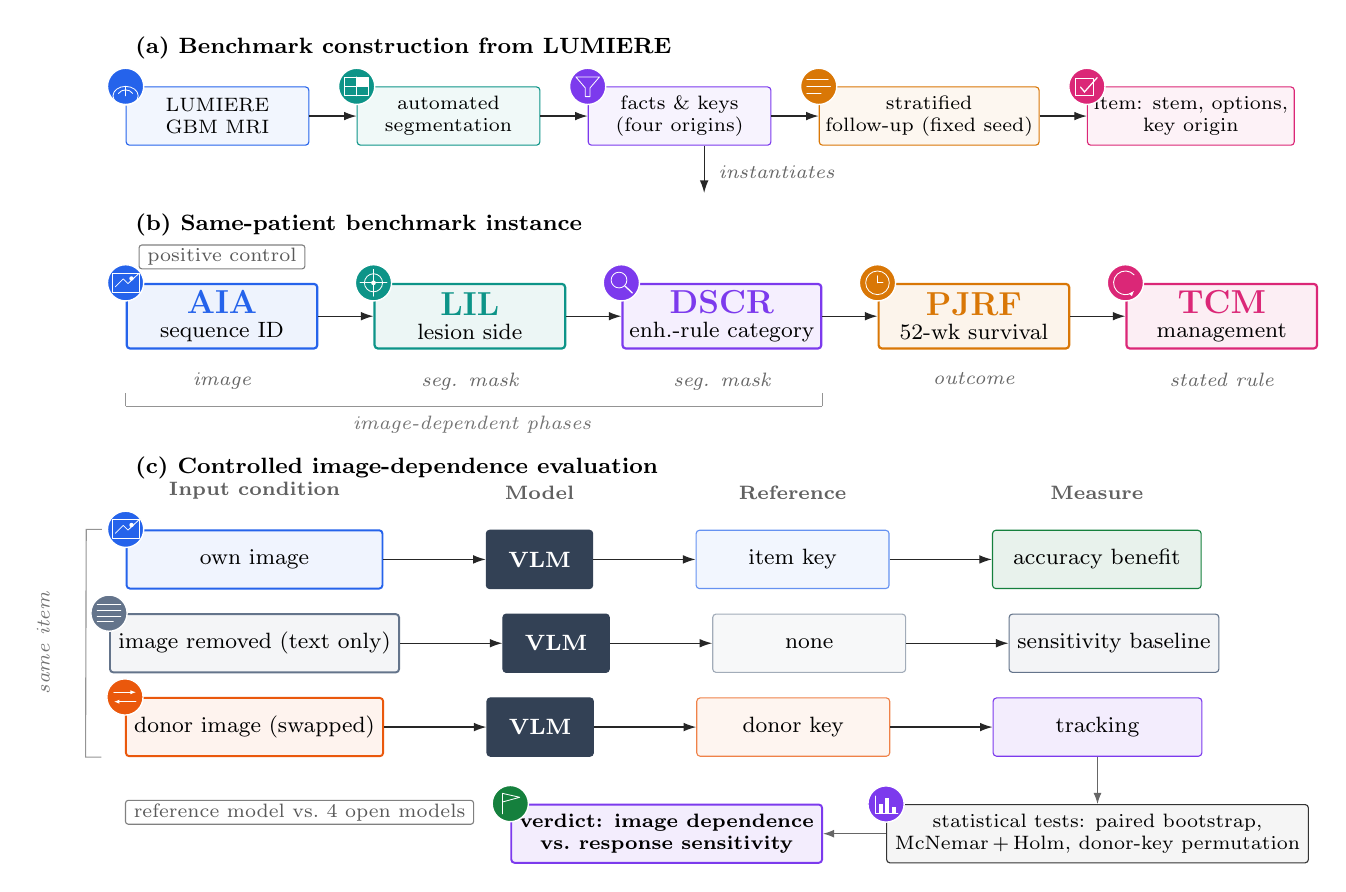
\begin{tikzpicture}[
    font=\footnotesize,
    >={Latex[length=1.6mm,width=1.1mm]},
    flow/.style={draw=black!85, line width=0.45pt, -{Latex[length=1.6mm,width=1.1mm]}},
    phase/.style={
        draw=black!82,
        rounded corners=1.2pt,
        minimum width=2.42cm,
        minimum height=0.82cm,
        align=center,
        inner sep=2.5pt,
        fill=white
    },
    imagephase/.style={phase, fill=black!4},
    sourcelabel/.style={font=\scriptsize\itshape, text=black!60, align=center},
    smalltag/.style={
        draw=black!50,
        rounded corners=1pt,
        fill=white,
        inner xsep=3pt,
        inner ysep=1.2pt,
        font=\scriptsize,
        text=black!65
    },
    rowbox/.style={
        draw=black!80,
        rounded corners=1.2pt,
        minimum width=3.25cm,
        minimum height=0.74cm,
        align=center,
        inner sep=3pt,
        fill=white
    },
    vlm/.style={
        draw=vlmcol,
        rounded corners=1.2pt,
        minimum width=1.35cm,
        minimum height=0.74cm,
        align=center,
        fill=vlmcol,
        text=white,
        font=\footnotesize\bfseries
    },
    refbox/.style={
        draw=black!70,
        rounded corners=1.2pt,
        minimum width=2.45cm,
        minimum height=0.74cm,
        align=center,
        inner sep=3pt,
        fill=white
    },
    measure/.style={
        draw=black!80,
        rounded corners=1.2pt,
        minimum width=2.65cm,
        minimum height=0.74cm,
        align=center,
        inner sep=3pt,
        fill=black!4
    },
    colhead/.style={font=\scriptsize\bfseries, text=black!62, align=center},
    paneltitle/.style={font=\footnotesize\bfseries, anchor=west},
    pipe/.style={
        draw=black!78,
        rounded corners=1.2pt,
        minimum width=2.32cm,
        minimum height=0.74cm,
        align=center,
        inner sep=2.2pt,
        fill=black!3,
        font=\scriptsize
    },
    analysisbox/.style={
        draw=black!80,
        rounded corners=1.2pt,
        minimum height=0.74cm,
        align=center,
        inner sep=3pt,
        fill=black!4,
        font=\scriptsize
    },
    verdictbox/.style={
        draw=dscrcol,
        line width=0.7pt,
        rounded corners=1.2pt,
        minimum height=0.74cm,
        align=center,
        inner sep=3pt,
        fill=dscrcol!9,
        font=\scriptsize\bfseries
    },
    branch/.style={draw=black!60, line width=0.4pt, -{Latex[length=1.4mm,width=1.0mm]}}
]

% ------------------------------------------------------------------
% (a) Benchmark construction pipeline
% ------------------------------------------------------------------
\node[paneltitle] (pp) at (0,0) {(a) Benchmark construction from LUMIERE};
\node[pipe, draw=aiacol, fill=aiacol!6, below=6mm of pp.south west, anchor=west] (src)
    {LUMIERE\\GBM MRI};
\node[pipe, draw=lilcol, fill=lilcol!6, right=6mm of src] (seg)
    {automated\\segmentation};
\node[pipe, draw=dscrcol, fill=dscrcol!6, right=6mm of seg] (fact)
    {facts \& keys\\(four origins)};
\node[pipe, draw=pjrfcol, fill=pjrfcol!6, right=6mm of fact] (samp)
    {stratified\\follow-up (fixed seed)};
\node[pipe, draw=tcmcol, fill=tcmcol!6, right=6mm of samp] (item)
    {item: stem, options,\\key origin};
\foreach \a/\b in {src/seg,seg/fact,fact/samp,samp/item}{\draw[flow] (\a) -- (\b);}
\ovbadgeat{src.north west}{aiacol}{brainic}
\ovbadgeat{seg.north west}{lilcol}{segic}
\ovbadgeat{fact.north west}{dscrcol}{factic}
\ovbadgeat{samp.north west}{pjrfcol}{sampleic}
\ovbadgeat{item.north west}{tcmcol}{itemic}

% ------------------------------------------------------------------
% (b) Same-patient benchmark instance
% ------------------------------------------------------------------
\node[paneltitle] (pa) at ([yshift=-10mm]src.south west) {(b) Same-patient benchmark instance};
\node[imagephase, draw=aiacol, line width=0.8pt, fill=aiacol!8, below=9mm of pa.south west, anchor=west] (aia) {
    {\large\bfseries\textcolor{aiacol}{AIA}}\\[-1pt]
    sequence ID
};
\node[imagephase, draw=lilcol, line width=0.8pt, fill=lilcol!8, right=7mm of aia] (lil) {
    {\large\bfseries\textcolor{lilcol}{LIL}}\\[-1pt]
    lesion side
};
\node[imagephase, draw=dscrcol, line width=0.8pt, fill=dscrcol!8, right=7mm of lil] (dscr) {
    {\large\bfseries\textcolor{dscrcol}{DSCR}}\\[-1pt]
    enh.-rule category
};
\node[phase, draw=pjrfcol, line width=0.8pt, fill=pjrfcol!8, right=7mm of dscr] (pjrf) {
    {\large\bfseries\textcolor{pjrfcol}{PJRF}}\\[-1pt]
    52-wk survival
};
\node[phase, draw=tcmcol, line width=0.8pt, fill=tcmcol!8, right=7mm of pjrf] (tcm) {
    {\large\bfseries\textcolor{tcmcol}{TCM}}\\[-1pt]
    management
};

\draw[flow] (aia) -- (lil);
\draw[flow] (lil) -- (dscr);
\draw[flow] (dscr) -- (pjrf);
\draw[flow] (pjrf) -- (tcm);

\node[sourcelabel, below=1.7mm of aia] {image};
\node[sourcelabel, below=1.7mm of lil] {seg. mask};
\node[sourcelabel, below=1.7mm of dscr] {seg. mask};
\node[sourcelabel, below=1.7mm of pjrf] {outcome};
\node[sourcelabel, below=1.7mm of tcm] {stated rule};

\node[smalltag, above=1.7mm of aia] {positive control};

% Minimal grouping cue for the image-dependent phases
\draw[black!42, line width=0.4pt]
  ([yshift=-7.2mm]aia.south west) -- ([yshift=-7.2mm]dscr.south east);
\draw[black!42, line width=0.4pt]
  ([yshift=-7.2mm]aia.south west) -- ++(0,1.7mm);
\draw[black!42, line width=0.4pt]
  ([yshift=-7.2mm]dscr.south east) -- ++(0,1.7mm);
\node[font=\scriptsize\itshape, text=black!55, anchor=north]
    at ($(aia.south)!0.5!(dscr.south)+(0,-7.2mm)$) {image-dependent phases};

% Colored icon badges (one per phase)
\ovbadgeat{aia.north west}{aiacol}{imgic}
\ovbadgeat{lil.north west}{lilcol}{targetic}
\ovbadgeat{dscr.north west}{dscrcol}{magic}
\ovbadgeat{pjrf.north west}{pjrfcol}{clockic}
\ovbadgeat{tcm.north west}{tcmcol}{cyclic}

% Feed arrow: construction pipeline instantiates the chain
\draw[flow] ($(src.south)!0.5!(item.south)$) -- ++(0,-6mm)
    node[pos=0.55, right=0.6mm, sourcelabel] {instantiates};

% ------------------------------------------------------------------
% (c) Controlled image-dependence evaluation
% ------------------------------------------------------------------
\node[paneltitle] (pb)
    at ([yshift=-15mm]aia.south west)
    {(c) Controlled image-dependence evaluation};

% Row 1: own image
\node[rowbox, draw=aiacol, line width=0.7pt, fill=aiacol!7, below=9mm of pb.south west, anchor=west] (own) {own image};
\node[vlm, right=13mm of own] (vlm1) {VLM};
\node[refbox, draw=aiacol!70, fill=aiacol!6, right=13mm of vlm1] (ref1) {item key};
\node[measure, draw=goodcol, fill=goodcol!10, right=13mm of ref1] (m1) {accuracy benefit};

% Column headers aligned to the actual columns
\node[colhead, above=2.6mm of own] {Input condition};
\node[colhead, above=2.6mm of vlm1] {Model};
\node[colhead, above=2.6mm of ref1] {Reference};
\node[colhead, above=2.6mm of m1] {Measure};

% Row 2: text only
\node[rowbox, draw=neutralcol, line width=0.7pt, fill=neutralcol!7, below=3.0mm of own] (text) {image removed (text only)};
\node[vlm, right=13mm of text] (vlm2) {VLM};
\node[refbox, draw=neutralcol!60, fill=neutralcol!5, right=13mm of vlm2] (ref2) {none};
\node[measure, draw=neutralcol, fill=neutralcol!8, right=13mm of ref2] (m2) {sensitivity baseline};

% Row 3: donor image
\node[rowbox, draw=swapcol, line width=0.7pt, fill=swapcol!7, below=3.0mm of text] (swap) {donor image (swapped)};
\node[vlm, right=13mm of swap] (vlm3) {VLM};
\node[refbox, draw=swapcol!75, fill=swapcol!6, right=13mm of vlm3] (ref3) {donor key};
\node[measure, draw=dscrcol, fill=dscrcol!9, right=13mm of ref3] (m3) {tracking};

% Arrows
\foreach \a/\b in {own/vlm1,vlm1/ref1,ref1/m1,text/vlm2,vlm2/ref2,ref2/m2,swap/vlm3,vlm3/ref3,ref3/m3}{
    \draw[flow] (\a) -- (\b);
}

% Colored icon badges (input conditions)
\ovbadgeat{own.north west}{aiacol}{imgic}
\ovbadgeat{text.north west}{neutralcol}{textic}
\ovbadgeat{swap.north west}{swapcol}{swapic}

% Same-item bracket
\draw[black!42, line width=0.4pt]
  ([xshift=-3mm]own.north west) -- ([xshift=-5mm]own.north west)
  -- ([xshift=-5mm]swap.south west) -- ([xshift=-3mm]swap.south west);
\node[rotate=90, font=\scriptsize\itshape, text=black!55, anchor=south]
  at ([xshift=-6.3mm]text.west) {same item};

% Reference-vs-open distinction (bottom-left, clear of the verdict)
\node[smalltag, anchor=west] (refopen) at ([yshift=-7mm]swap.south west) {reference model vs.\ 4 open models};

% Analysis branches: the three measures feed the tests, then the verdict
\node[analysisbox, minimum width=3.9cm, below=6mm of m3] (tests)
  {statistical tests: paired bootstrap,\\McNemar\,$+$\,Holm, donor-key permutation};
\node[verdictbox, minimum width=3.0cm, left=8mm of tests] (verdict)
  {verdict: image dependence\\vs.\ response sensitivity};
\draw[branch] (m3.south) -- (tests.north);
\draw[branch] (tests.west) -- (verdict.east);
\ovbadgeat{tests.north west}{dscrcol}{chartic}
\ovbadgeat{verdict.north west}{goodcol}{flagic}

\end{tikzpicture}
\caption{Evaluation overview. (a) Construction: a LUMIERE glioblastoma case becomes items through automated segmentation, fact extraction from the images, masks and records, stratified sampling of one follow-up, and item assembly; the keys have four origins (AIA sequence, LIL and DSCR segmentation, PJRF outcome, TCM rule). (b) The item instantiates a five-phase same-patient chain; the image-dependent phases (AIA, LIL, DSCR) carry the keys tested here and AIA is the positive control. (c) Each image-dependent phase is run under three controlled input conditions, the patient's own image, text only, and a donor-image swap, giving an accuracy benefit, a response-sensitivity baseline, and a donor-tracking measure; these feed the statistical tests and the image-dependence-versus-response-sensitivity verdict. A reference model is a positive control alongside the four open-weight models.}
\label{fig:overview}
\end{figure*}


\section{Related Work}
\label{sec:related-work}

\paragraph{Shortcuts and faithfulness.} Models can reach correct labels without performing the intended reasoning. Hypothesis-only baselines exploit annotation artifacts in NLI datasets \citep{poliak2018hypothesis,gururangan2018annotation}, models adopt heuristics that fail on HANS \citep{mccoy2019right}, and biased input features can alter chain-of-thought answers without appearing in the stated rationale \citep{turpin2023language}.

\paragraph{Answering without the image.} Visual question-answering models often exploit language priors. \citet{goyal2017making} countered this by pairing questions with images yielding different answers, while \citet{chen2024right} show that many multimodal benchmark items do not require visual content. Similar failures appear in medicine: \citet{yan2025worse} report severe degradation under adversarial diagnostic counterparts, \citet{jin2024hidden} find flawed rationales in 35.5\% of GPT-4V's correct answers, and \citet{nguyen2025localizing} (HEAL-MedVQA) use textual and visual perturbations to localize shortcuts in chest-radiograph QA. We extend this logic to brain-MRI questions. HEAL-MedVQA \citep{nguyen2025localizing} already replaces a pathological region with a corresponding region from a different-class image and scores the expected answer transition; our increment is in the intervention unit and the inference, not the idea of a counterfactual image. We swap the whole image for a different patient's, score against the donor's key across all classes with the no-image donor-key agreement subtracted, and add per-phase reference values, a conditional donor-label association test, and a rule--expert agreement audit motivating the targets. Concurrent evaluations probe medical VQA with blank, shuffled or mismatched images and report answer similarity or sensitivity \citep{zafar2026beyond, zhu2026ask4vg}; we instead score the swapped answer against the donor's key across all classes with the no-image agreement subtracted. Unlike correctness on complementary pairs \citep{goyal2017making}, which requires the model to answer each image correctly, this statistic measures movement toward what the swapped image supports and so is informative even for models that are rarely correct, as ours are. We did not run HEAL-MedVQA's protocol, so the comparison is one of design and we claim no empirical superiority. The combination adds discrimination a raw gain lacks: a non-specific image shift and a noisy tracker both reach \vfourDonorValShiftGain{} points of gain and change a comparable share of answers, yet the conditional donor-label permutation flags them at \vfourDonorValShiftDetect{}\% and \vfourDonorValTrackLowDetect{}\% (Table~\ref{tab:donorval}). The same-patient chain extends the questions to interventions on supplied clinical facts. UniMod \citep{gu2026unimod} addresses modality imbalance during training by supervising image-only, text-only, and fused predictions separately; we instead evaluate existing models for observable image dependence.

\paragraph{Brain benchmarks and longitudinal data.} OmniBrainBench \citep{peng2026omnibrainbench} contains 6,823 closed-ended brain-imaging questions spanning five clinical phases and 15 modalities. Its supplement describes a patient-level ADNI extension, but we did not evaluate it. LUMIERE \citep{suter2022lumiere} and MU-Glioma-Post \citep{muglioma2025post} provide longitudinal glioma imaging, treatment, and outcome data but no question layer.





\section{Building Chains from LUMIERE}
\label{sec:lumiere}

\paragraph{Why not OmniBrainBench.} A chain needs one patient's phases. We checked whether any image is shared across questions of different phases within a grouped case: of 6,823 closed-ended questions only 2 verifiable cross-phase patient links exist, and a second method based on filename identifiers agreed; the counts are lower bounds. Each sub-corpus was built for one task, so a patient is essentially asked one phase-type of question. This is an incompatibility between the released groupings and our evaluation, not a defect in a promise its authors made.

\paragraph{LUMIERE.} LUMIERE \citep{suter2022lumiere} has 91 glioblastoma patients with longitudinal MRI (T1, contrast-enhanced T1, T2, FLAIR), automated segmentations (DeepBraTumIA and HD-GLIO-AUTO; \citealp{suter2022lumiere, kickingereder2019automated}), RANO ratings by one neuroradiologist \citep{wen2010updated}, and overall survival for most patients. Segmentations are automated and were not manually verified; the ratings are expert-assigned.

\subsection{Motivating audit: can an automated rule reproduce the expert ratings from the displayed slices?}
\label{sec:audit}

The natural key for a diagnosis-category question is the expert RANO rating, but whether it can be recovered from the displayed slices is untested, so we ran an automated agreement audit: for each first-line follow-up we tracked one enhancing lesion across scans, measured it on its own largest axial cross-section, computed the RANO bidimensional product and applied the enhancement criteria (progression: measurable disease at least 25\% above the nadir, the smallest earlier measurement, or measurable disease where the nadir had none; response against the post-operative baseline; measurable means both diameters at least 10 mm). The rule has no new-lesion criterion beyond that. Its nadir handling and abstention were fixed after inspecting agreement with the expert ratings and before item building, so this agreement is not independent of rule development (tuning toward agreement would, if anything, raise it). Coverage: of \vfourFollowups{} first-line follow-ups, \vfourUndetermined{} are undetermined because no measurable enhancing disease exists on the baseline or nadir scan, so the rule abstains. Agreement, our primary number, is over the \vfourDeterminate{} determinate follow-ups: the rule reproduces the expert category for \vfourConcordant{} (\vfourConcordantDetPct{}\%, Wilson 95\% interval \vfourConcordantDetLo{} to \vfourConcordantDetHi{}\%, and \vfourAuditClusterLo{} to \vfourAuditClusterHi{}\% when the \vfourAuditPatients{} patients are resampled; counting the undetermined as failures would give \vfourConcordantPct{}\%, mixing abstention with disagreement). Most of the \vfourDisagree{} disagreements are the rule returning complete response where the expert rated progressive or stable disease. Disagreement has several sources this audit does not separate; LUMIERE records that one neuroradiologist rated the studies but not what they used, and our automated product correlates only moderately with the rater's recorded target-lesion diameters (Spearman \vfourBpRho{} over \vfourBpN{} follow-ups), so measurement error is one plausible contributor. The audit thus shows disagreement without establishing which procedure is wrong or how many items are unanswerable, which would need qualified reviewers on a sample of the disagreements.

\subsection{The item set}
\label{sec:v4}

The keys have four different origins (Table~\ref{tab:phases}), and we make no uniform claim that each is a function of what the model sees: AIA is the sequence rendered; LIL and DSCR are derived from automated segmentation masks the model does not see (recoverable from the slices only if the segmentation is right; these are segmentation-derived targets reviewers have not validated); PJRF is the recorded outcome, scored probabilistically since a future outcome is not a function of the stated facts; and TCM is the output of a stated management rule, testing adherence rather than clinical correctness. All random choices use fixed seeds and never look at model output.

\begin{table*}[t]
\centering
\footnotesize
\setlength{\tabcolsep}{3pt}
\begin{tabular}{p{1.3cm}p{4.1cm}p{4.4cm}p{4.4cm}r}
\toprule
\hdrrow Phase & Question & Model-visible inputs & Key & $n$ \\
\midrule
\ptagAIA & Which MRI sequence is shown? & one axial slice (T1, T1 after contrast, T2 or FLAIR) & the sequence rendered & \vfourNAIA{} \\
\bandrow \ptagLIL & Hemisphere and anterior/posterior half of the main tumor region & follow-up contrast-enhanced T1 slice at the level of the largest tumor region & position of the largest tumor-core component on that slice, relative to the midline and the brain's front-to-back midpoint & \vfourNLIL{} \\
\ptagDSCR & Simplified enhancement-rule category at follow-up (exploratory) & baseline, follow-up and (when different from the baseline) nadir slices at the largest cross-section of the tracked enhancing lesion; the thresholds are stated & category from the bidimensional products of the single tracked enhancing component on those slices & \vfourNDSCR{} \\
\bandrow \ptagPJRF & Probability of death within 52 weeks of this scan & age, sex, MGMT, IDH, extent of resection, weeks since surgery; alive at the scan & recorded outcome; scored by Brier score, not accuracy & \vfourNPJRF{} \\
\ptagTCM & Next management step & the same clinical facts plus weeks since chemoradiotherapy; the category comes from the chain & rule: non-PD continue; PD within 12 weeks of radiotherapy repeat MRI first; PD later change therapy & \vfourNTCM{} \\
\bottomrule
\end{tabular}
\caption{The phases. Stems for AIA, LIL and DSCR contain no patient-specific fact and every option set contains every possible answer, so a swapped image never conflicts with the text and the donor's answer is always available. DSCR shows two images, or three when the nadir differs from the baseline.}
\label{tab:phases}
\end{table*}

\paragraph{Cohort.} We select one first-line follow-up per patient (before any second surgery), in strata defined by the TCM rule class and the DSCR category, with quotas and seed fixed in advance, giving \vfourPatients{} patients. Within each stratum, eligible follow-ups were ranked to prefer agreement between the automated rule category and the expert rating, then LIL eligibility, with seeded random tie-breaking. This enriches the selected set for rule--expert agreement: it contains \vfourSelectedAgree{} of \vfourPatients{} agreements (\vfourSelectedAgreePct{}\%), against \vfourConcordantDetPct{}\% across the \vfourDeterminate{} determinate audit follow-ups; the two rates have different sampling units and are not an unbiased before/after effect, so this enrichment limits population-level interpretation. Selection used tabular records and segmentation masks only and no model output, and progressive-disease follow-ups within 2 weeks of the 12-week window are left out.

\paragraph{Images.} Each image is an atlas-space axial slice, skull-stripped by the dataset authors with HD-BET \citep{isensee2019automated}, at 4$\times$ magnification with a 20\,mm scale bar, in radiological orientation. Slice levels are those on which the key is computed.

\paragraph{AIA, LIL, DSCR.} AIA is the positive control: its key is the sequence rendered, balanced over four sequences (the most common covers \vfourMajorityAIA{}\% of items), so text alone can reach only chance in expectation. LIL's key is the hemisphere and anterior/posterior half of the largest tumor-core component on the displayed slice; lesions within 10\,mm of a midline, smaller than 100\,mm$^2$ or with under 80\% of their pixels on their centroid's side of the midline are not asked about. DSCR's stem states the enhancement criteria, and its key is the category computed from the bidimensional products of a single tracked enhancing component (the one nearest the baseline target lesion). The stem's phrase ``a new measurable enhancing lesion'' refers to that tracked component becoming measurable from a non-measurable nadir; a separate new lesion elsewhere is not scored, and the key does not implement a general new-lesion search (see Limitations). Because the key is this simplified single-component rule rather than validated clinical RANO, we treat DSCR as an exploratory agreement task against a mechanically defined proxy, and read AIA and LIL as the strongest image-dependence demonstrations.

\paragraph{PJRF.} The prediction time is the follow-up scan and the outcome is death within 52 weeks of it, from the LUMIERE survival record. The model picks one of four probability bins (midpoints .10, .30, .50, .80) and is scored with the Brier score, not by whether it picked a ``correct'' bin. The base rate (Table~\ref{tab:baselines}) reflects our selection, not a population rate. The origin and censoring of the survival time are undocumented, so PJRF is secondary and no other claim in this paper rests on it.

\paragraph{TCM.} LUMIERE records no treatment after chemoradiotherapy, so a documented treatment is not available and the key is a rule-based recommendation, not what was done: non-progressive disease continues adjuvant temozolomide; progressive disease within 12 weeks of completing radiotherapy is confirmed with repeat MRI before any change; later progressive disease prompts a change of therapy. The base stems supply the clinical facts but not this rule; only a post hoc condition states the rule in the prompt (Section~\ref{sec:results}). The 12-week window is from the RANO criteria \citep{wen2010updated}; because we cannot assess the radiation field, the rule is a simplification (see Limitations). Radiotherapy dates are not in LUMIERE, so the stem states the weeks since chemoradiotherapy under an assumed standard schedule (ending 10 weeks after surgery). The same diagnosis therefore maps to different actions depending on the stated timing (\vfourTcmConfirm{} repeat-MRI and \vfourTcmEscalate{} change-therapy items among \vfourTcmPdItems{} progressive-disease items), which lets a lookup of the category alone be told apart from use of the timing fact.




\section{Controls and Pre-specified Analysis}
\label{sec:controls}

The target is \emph{correct, task-relevant image dependence under specified interventions}: whether a model's answer moves toward what the displayed image supports, not merely whether its output reacts to the image. Majority-baseline performance is contextual evidence for an accuracy gain, not a necessary test for image use: a model can read some items from the slice yet still score below the most common key by missing others, so accuracy below that share neither establishes nor refutes image use on its own.

The analysis plan (hypotheses, margin, correction family, seeds and decision rules) is an internal prespecified plan written before any model run and provided in that repository; it is not externally timestamped. It was amended twice after an initial run: correcting two key-construction measurement errors reduced the cohort from 62 to 46 patients and every condition was rerun on the corrected items, and a later correction to the DSCR stem wording prompted a rerun of the conditions that display it (first-round runs are not reported). The hypotheses, margin, correction family, seeds and decision rules were unchanged.

Models are the four open-weight models (MedGemma-4B \citep{sellergren2025medgemma}, Gemma-3-12B and Gemma-3-27B \citep{gemmateam2025gemma3}, Llama-4-Scout; 4-bit, greedy decoding, 800 tokens; the reference model uses 16{,}384 tokens because hidden reasoning counts against the cap; unparseable responses score incorrect). Each condition asks one question with a manufactured upstream context, so a phase's effect is not mixed with the model's own earlier answers.

\begin{itemize}[leftmargin=*, itemsep=1pt, topsep=2pt]
    \item \textbf{E1, image effect} (AIA, LIL, DSCR): accuracy with the image minus text only, paired by patient, with a patient-bootstrap interval. The margin is $\pm10$ percentage points, fixed in advance; ``within margin'' requires the whole interval inside it, which at these sample sizes is reachable only when few items differ between the arms. Holm correction over the 12 model-phase tests; other contrasts are descriptive and unadjusted, with exact McNemar tests \citep{mcnemar1947note} and Wilson intervals \citep{wilson1927probable} where a proportion is reported. Because the bootstrap collapses to zero width when every pair is concordant, we also report, post hoc, an add-half interval for the paired difference \citep{agresti2005simple} and the exact $p$. \textbf{AIA is the positive control:} the plan's operational reading rule is that for a model whose unadjusted AIA interval is not above zero, the test has not been shown to detect image use, and E1 on LIL and DSCR supports no conclusion about it.
    \item \textbf{E2, donor tracking}: swap the image for a donor's with a different key (one donor per patient and phase, same number of images); $G=1[\text{swap}=\text{donor key}]-1[\text{text only}=\text{donor key}]$, so the no-image prior is subtracted. The estimand is conditional on the fixed assignment, in which a patient donates to at most two recipients. Because a positive gain can come from a generic response to any image rather than from the shown donor, we add a post hoc \emph{conditional label-association} permutation: holding each recipient's observed answers fixed, it treats the assigned donor-key labels as exchangeable among recipients within each equal-image-count stratum, keeping a reused donor's recipients together, subject to the swap constraint that no recipient receives its own key, and asks whether answers match the assigned donor's key more often than a key drawn from a different donor. It does not reconstruct the image-assignment mechanism, so it licenses only that narrow comparison. The reference distribution is generated by assigning the constrained donor-key labels sequentially in random block order, which is constraint-valid but not exactly uniform over all admissible allocations; its calibration below therefore applies to the synthetic nulls evaluated here, and it is not a uniform conditional permutation test or a randomization test for the original image-assignment mechanism. On synthetic predictors with known behaviour, the permutation flags a genuine tracker but not a generic image-presence shift and holds its false-positive rate at the nominal 5\% under this constraint-valid no-tracking null (Table~\ref{tab:donorval}; the Type-I calibration of this permutation is in the repository).
    \item \textbf{E3, use of stated facts} (TCM): with the true context, move the stated timing across the 12-week window (\emph{flip\_window}) or replace the stated category by one that maps to another action class (\emph{flip\_label}). The prespecified summary was the share of answers equal to the rule's new answer; because that counts answers that had not changed, we instead report each item's transition relative to the true-context answer and take moved over informative items as the rate of interest. A category lookup alone reaches at most \vfourTcmLookupEsc{}\% accuracy (\vfourTcmLookupConf{}\% if it always confirms first) and cannot follow the timing flip.
    \item \textbf{E4, upstream context}: true, randomly wrong (a seeded incorrect option per earlier answer), or absent context.
    \item \textbf{E5, PJRF} (secondary; results in the repository): Brier score and skill against the leave-one-out base rate, and AUC.
\end{itemize}

We report three observable outcomes separately: accuracy benefit (E1), output sensitivity (the share of items whose answer letter differs between the image and text-only arms, and between the swapped and own image), and correct donor tracking (E2); none observes internal processing. Output sensitivity, the transition tables and the output-handling counts are post hoc, descriptive analyses. The ordinary five-phase chain (own answers as context) is run with and without images as a secondary analysis; each arm regenerates its upstream answers, so later-phase differences are total effects through the chain.

\paragraph{Reference and precision controls.} Three of the four open models did not meet the operational AIA gate (Section~\ref{sec:results}), so we added three post hoc controls, each reported apart from the four-model Holm family and run under the same prompts, temperature 0 and decision rules. (i)~A reference (positive-control) model, Gemini-3.6-Flash, on E1 and E2; empty API responses are counted and rerun before results are read (none occurred: \vfourCtrlEmpty{} of \vfourCtrlRecords{} records), and, being an API model, it can change without notice. (ii)~A precision control, Gemma-3-27B rerun in bf16; its reading rule, fixed in advance, attributed part of the gap to quantization only if the bf16 AIA interval rose clearly above the 4-bit model's, but the serving stack also differs from the Ollama runs, so precision and stack are confounded (we draw no conclusion). (iii)~A non-Gemma control, Pixtral-12B (bf16), on E1 and E2 for AIA and LIL; its DSCR image conditions are excluded post hoc because the three-image prompt returned empty output for many records.


\section{Results}
\label{sec:results}

\subsection{Reference values without a model}

Table~\ref{tab:baselines} gives what constants and lookups reach. AIA is close to uniform over four answers, DSCR's most common category is progressive disease for \vfourMajorityDSCR{}\% of items, and a category-only TCM lookup reaches at most \vfourTcmLookupEsc{}\%.

\begin{table}[t]
\centering
\footnotesize
\setlength{\tabcolsep}{3pt}
\begin{tabular}{lrrl}
\toprule
\hdrrow Phase & $n$ & Chance & Most common key \\
\midrule
\ptagAIA & \vfourNAIA{} & 25.0 & \vfourMajorityAIA{}\% \\
\bandrow \ptagLIL & \vfourNLIL{} & 25.0 & \vfourMajorityLIL{}\% \\
\ptagDSCR & \vfourNDSCR{} & 25.0 & \vfourMajorityDSCR{}\% \\
\bandrow \ptagTCM & \vfourNTCM{} & 25.0 & \vfourMajorityTCM{}\% (lookup $\le$ \vfourTcmLookupEsc{}\%) \\
\ptagPJRF & \vfourNPJRF{} & (Brier) & base rate \vfourPjrfBase{}\% \\
\bottomrule
\end{tabular}
\caption{Non-model references on the items: chance, share of the most common key, the ceiling of a category-only TCM lookup, and the PJRF base rate.}
\label{tab:baselines}
\end{table}

\subsection{Image controls and stated facts}

\begin{table*}[t]
\centering
\scriptsize
\setlength{\tabcolsep}{2pt}
\begin{tabular}{llrrrlrl}
\toprule
Model & Phase & $n$ & Image & Text-only & $\Delta$ [95\% CI] & Answers differ & Interval \\
\midrule
MedGemma-4B & AIA & 46 & 34.8 & 26.1 & +8.7 [$-$2.2, +21.7] & 30.4 & inconclusive \\
MedGemma-4B & LIL & 38 & 23.7 & 18.4 & +5.3 [$-$5.3, +15.8] & 18.4 & inconclusive \\
MedGemma-4B & DSCR & 46 & 19.6 & 10.9 & +8.7 [+2.2, +17.4] & 19.0 & CI above 0 \\
Gemma-3-12B & AIA & 46 & 26.1 & 26.1 & +0.0 [$-$13.0, +13.0] & 32.6 & inconclusive \\
Gemma-3-12B & LIL & 38 & 31.6 & 23.7 & +7.9 [$-$7.9, +23.7] & 47.4 & inconclusive \\
Gemma-3-12B & DSCR & 46 & 58.7 & 47.8 & +10.9 [+2.2, +19.6] & 11.9 & CI above 0 \\
Gemma-3-27B & AIA & 46 & 32.6 & 26.1 & +6.5 [$-$2.2, +17.4] & 26.1 & inconclusive \\
Gemma-3-27B & LIL & 38 & 23.7 & 18.4 & +5.3 [$-$5.3, +15.8] & 34.2 & inconclusive \\
Gemma-3-27B & DSCR & 46 & 58.7 & 58.7 & +0.0 [+0.0, +0.0] & 0.0 & within $\pm$10 pp \\
Llama-4-Scout & AIA & 46 & 37.0 & 23.9 & +13.0 [+2.2, +26.1] & 30.4 & CI above 0 \\
Llama-4-Scout & LIL & 38 & 39.5 & 34.2 & +5.3 [$-$10.5, +21.1] & 44.7 & inconclusive \\
Llama-4-Scout & DSCR & 46 & 54.3 & 8.7 & +45.7 [+28.3, +63.0] & 88.1 & CI above 0 \\
\bottomrule
\end{tabular}

\caption{E1: accuracy (\%) with the image and text only (no upstream context), the paired difference in points with its bootstrap interval, an add-half sparse-data interval (Add-half CI), the exact McNemar $p$ (unadjusted), the share of items whose answer differs between the two arms (answers differ), and the interval reading. The interval reading is descriptive; Holm-corrected exact McNemar tests determine confirmatory significance (only Llama-4-Scout on DSCR survives). Gemma-3-27B gives a constant class in both DSCR arms, so its within-margin label rests on the add-half interval. Answers-differ is over items in all three arms (AIA 46, LIL 38, DSCR 42 of 46); accuracy is over all items per phase (AIA 46, LIL 38, DSCR 46). AIA is the positive control.}
\label{tab:e1}
\end{table*}


\paragraph{The reference model reads the image.} Gemini-3.6-Flash identifies the sequence for \vfourEoneOwnAIAGemini{}\% of patients with the image and \vfourEoneTextAIAGemini{}\% without (difference \vfourEoneDiffAIAGemini{} points, 95\% CI [\vfourEoneLoAIAGemini{}, \vfourEoneHiAIAGemini{}]), places the lesion for \vfourEoneOwnLILGemini{}\% against \vfourEoneTextLILGemini{}\%, and with the image swapped gives the donor's answer for \vfourEtwoSwapAIAGemini{}\% (AIA) and \vfourEtwoSwapLILGemini{}\% (LIL) of patients (Table~\ref{tab:ctrl}). A model that reads the slices can therefore answer these items, so the tasks are feasible; this does not show that every item is valid, nor why a weaker model fails. DSCR is different: the reference model scores \vfourEoneOwnDSCRGemini{}\% with the image and \vfourEoneTextDSCRGemini{}\% without, where the most common key covers \vfourMajorityDSCR{}\% of items, so most of its text-only accuracy is the class prior and it recovers the key for only \vfourEoneOwnDSCRGemini{}\% of items. We therefore cannot establish that DSCR is answerable from the slices for every item (the shortfall may be perception, keys the model does not see, or key error), so a null DSCR effect for another model cannot be read as a failure to use the image.

\paragraph{Open models: image effect (E1).} Sequence identification stays between \vfourEoneOwnAIAGemmaTwelve{} and \vfourEoneOwnAIAScout{}\% (chance 25\%); Table~\ref{tab:e1} gives every cell and the per-model effect with its interval. The operational AIA gate (an unadjusted interval above zero) is met only by Llama-4-Scout, and only on the bootstrap interval (exact McNemar $p=\vfourEonePAIAScout{}$). No conclusion depends on this borderline pass: the gate is a conservative screen, not a prerequisite for lesion or category reading, so the DSCR case below is read through the additions, and the limited evidence of open-model image dependence holds whether or not Scout passes. One image-effect test survives Holm correction, Llama-4-Scout on DSCR, but it does not show the model reads the category from the slices: its accuracy with the image stays below the most common key's share (\vfourMajorityDSCR{}\%) and its text-only accuracy far below, so the difference gives the gap, not its mechanism. This below-majority accuracy is not a constant answer: class-wise (Table~\ref{tab:confusion}), Scout answers \vfourConfOnMajority{} of \vfourConfOnMajorityN{} progressive-disease items and recovers \vfourConfOffMajority{} of \vfourConfOffMajorityN{} non-majority items (complete-response recall \vfourConfRecallCR{}\%, stable-disease \vfourConfRecallSD{}\%), so scoring below the majority share reflects redistributed errors, not non-use of the image. In the prespecified sensitivity analysis restricted to the \vfourSensSubN{} items whose rule category also equals the expert rating (\vfourSensSubMajPct{}\% progressive disease), Llama-4-Scout's difference is \vfourSensSubDiffScout{} points [\vfourSensSubLoScout{}, \vfourSensSubHiScout{}], still below that subset's majority share, and the reference model's is 0.0 (\vfourSensSubRefAcc{}\% with the image and text only). The DSCR intervals above zero for MedGemma-4B and Gemma-3-12B do not survive correction; on LIL every interval includes zero. A test that fails correction is not evidence of no effect: no open-model AIA or LIL interval lies inside the $\pm10$-point margin. Each open model's AIA answers concentrate on one sequence (modal answer \vfourAiaModalShareLo{} to \vfourAiaModalShareHi{}\% of the \vfourNAIA{} items), consistent with a fixed default under weak image use.

\paragraph{Precision control.} Rerun in bf16, Gemma-3-27B identifies the sequence for \vfourEoneOwnAIAGemmaTwentySevenBf{}\% with the image and \vfourEoneTextAIAGemmaTwentySevenBf{}\% without (against \vfourEoneOwnAIAGemmaTwentySeven{}\% at 4-bit in Table~\ref{tab:e1}): the interval includes zero, so the rerun did not restore AIA performance, and its LIL and DSCR intervals also include zero (precision and stack are confounded, so we draw no conclusion). A different-family bf16/vLLM model, Pixtral-12B, is likewise near chance on sequence (\vfourEoneOwnAIAPixtral{}\% against \vfourEoneTextAIAPixtral{}\%) and lesion side, with no detected donor tracking (DSCR image arms excluded), so 4-bit Ollama serving is an unlikely sole cause, though scale and training still differ.

\paragraph{Open models: donor tracking (E2).} Swapping the image changes a substantial share of AIA and LIL answers (Table~\ref{tab:e2}), but the new answer follows the donor's key with an interval above zero in only two cells: MedGemma-4B on AIA (gain \vfourEtwoGainAIAMedGemma{}; exact $p=\vfourEtwoPAIAMedGemma{}$) and Llama-4-Scout on DSCR (\vfourEtwoGainDSCRScout{}; $p=\vfourEtwoPDSCRScout{}$), the phase in which its accuracy gain also survives correction. Both cells therefore meet the prespecified E2 criterion (gain interval above zero). Because a generic response to any image can also produce a positive gain (Table~\ref{tab:donorval}), we added the post hoc permutation below and interpret the cells by it rather than by the prespecified rule; the Holm correction over the E2 cells is likewise post hoc. Both survive resampling by donor and dropping any one donor. Llama-4-Scout on DSCR is not separable from a random assignment of donor keys (permutation $p=\vfourDonorPermDSCRScout{}$); MedGemma-4B on AIA reaches a raw permutation $p=\vfourDonorPermAIAMedGemma{}$ but does not survive Holm correction over the twelve open-model cells ($p=\vfourStratHolmAIAMedGemma{}$) and fails the AIA positive-control gate, so we read neither as donor-specific tracking. Under that permutation a random assignment of donor keys yields a mean gain of about \vfourDonorNullMeanDSCRScout{} points, so most of Scout's gain of \vfourEtwoGainDSCRScout{} points is expected without donor-specific reading. The same association logic applied to the own-image arm (keys permuted within image-count strata, answers fixed; post hoc) gives a weak Scout DSCR association ($\kappa=\vfourOwnKappaDSCRScout{}$, unadjusted $p=\vfourOwnPDSCRScout{}$; text-only control $p=\vfourOwnTextPDSCRScout{}$) that does not survive Holm over the twelve cells ($p=\vfourOwnHolmDSCRScout{}$), so category reading is suggested but not established. Across \vfourRobustScoutNAssign{} re-drawn valid donor assignments Scout's DSCR gain ranges \vfourRobustScoutDSCRGainMin{} to \vfourRobustScoutDSCRGainMax{} points yet the permutation is significant in none of them ($p$ from \vfourRobustScoutDSCRPermPMin{} to \vfourRobustScoutDSCRPermPMax{}), so donor-specific tracking is not detected under any assignment, while the reference model's AIA and LIL permutations stay significant under every assignment (its DSCR swap was not rerun under alternative assignments). Every other interval includes zero, and the open-model sequence and lesion-side gains are far below the reference model's (Table~\ref{tab:ctrl}).

\begin{figure}[t]
\centering
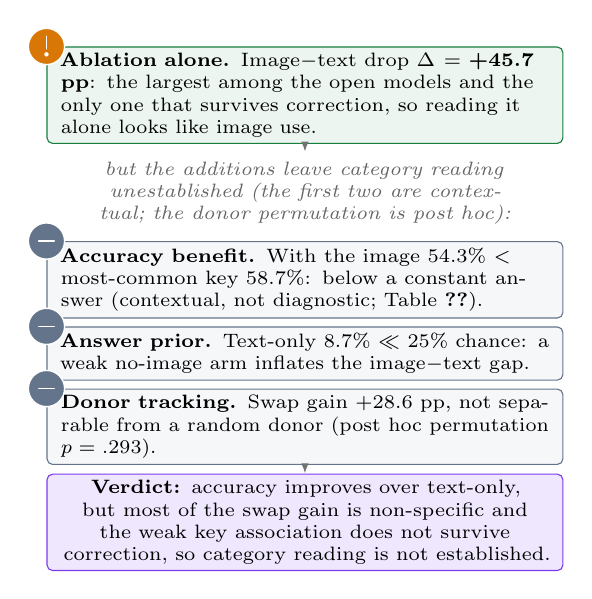
\begin{tikzpicture}[
  font=\scriptsize,
  card/.style={draw, rounded corners=2pt, text width=62mm, align=left, inner xsep=5pt, inner ysep=2.3pt},
  conn/.style={-{Latex[length=1.3mm]}, black!55, semithick},
]
% The tempting reading
\node[card, draw=goodcol, fill=goodcol!8] (temp)
  {\textbf{Ablation alone.} Image$-$text drop $\Delta=$ \textbf{\vfourEoneDiffDSCRScout{} pp}: the largest among the open models and the only one that survives correction, so reading it alone looks like image use.};
\node[below=1.0mm of temp.south, font=\scriptsize\itshape, text=black!60, text width=62mm, align=center] (but)
  {but the additions leave category reading unestablished (the first two are contextual; the donor permutation is post hoc):};
% Three failing controls
\node[card, draw=neutralcol, fill=neutralcol!6, below=0.9mm of but] (c1)
  {\textbf{Accuracy benefit.} With the image \vfourEoneOwnDSCRScout{}\% $<$ most-common key \vfourMajorityDSCR{}\%: below a constant answer (contextual, not diagnostic; Table~\ref{tab:confusion}).};
\node[card, draw=neutralcol, fill=neutralcol!6, below=1.0mm of c1] (c2)
  {\textbf{Answer prior.} Text-only \vfourEoneTextDSCRScout{}\% $\ll$ 25\% chance: a weak no-image arm inflates the image$-$text gap.};
\node[card, draw=neutralcol, fill=neutralcol!6, below=1.0mm of c2] (c3)
  {\textbf{Donor tracking.} Swap gain \vfourEtwoGainDSCRScout{} pp, not separable from a random donor (post hoc permutation $p=\vfourDonorPermDSCRScout{}$).};
% Verdict
\node[card, draw=dscrcol, fill=dscrcol!12, below=1.1mm of c3, align=center, text width=62mm] (v)
  {\textbf{Verdict:} accuracy improves over text-only, but most of the swap gain is non-specific and the weak key association does not survive correction, so category reading is not established.};
\draw[conn] (temp.south) -- (but.north);
\draw[conn] (c3.south) -- (v.north);
% Badges
\ovbadgeat{temp.north west}{pjrfcol}{bangic}
\ovbadgeat{c1.north west}{neutralcol}{dashic}
\ovbadgeat{c2.north west}{neutralcol}{dashic}
\ovbadgeat{c3.north west}{neutralcol}{dashic}
\end{tikzpicture}
\caption{Worked example (Llama-4-Scout, DSCR): the ablation drop, largest among the open models and surviving correction, would alone credit image use, but the additions (accuracy benefit over the answer prior, the prior itself, and donor tracking, the last assessed by a post hoc permutation) do not establish that the category is read from the slice. Below-majority accuracy does not by itself rule out item-level image reading; the donor-association result is a separate, conditional diagnostic.}
\label{fig:worked}
\end{figure}

\paragraph{Worked example.} Figure~\ref{fig:worked} works Llama-4-Scout on DSCR through the controls: the largest ablation drop among the open models, and the only one to survive correction, shows response sensitivity to the image, but the accuracy benefit, the answer prior and the post hoc donor permutation ($p=\vfourDonorPermDSCRScout{}$, not separable from a random assignment) leave correct category reading unestablished.

\paragraph{Stated facts and context (E3, E4; extension).} The main TCM condition measures agreement with a simplified policy that is not supplied in the prompt; only the post hoc explicit-rule condition below tests adherence to a supplied policy. With the true context, main-condition accuracy is below the best category-only lookup (\vfourTcmLookupEsc{}\%) for all four open models, though Gemma-3-12B and Gemma-3-27B exceed the confirm-first lookup (\vfourTcmLookupConf{}\%); this lookup is a sample oracle, not a held-out baseline, so the comparison is descriptive. Reading each item against itself, replacing the stated category moves the answer for a minority of informative items in three models and a slim majority in Gemma-3-27B (\vfourTransLabelMovedGemmaTwentySeven{} of \vfourTransLabelInfGemmaTwentySeven{}); crossing the 12-week window moves it most for Llama-4-Scout and for none of Gemma-3-27B's \vfourTransTimingInfGemmaTwentySeven{} informative progressive-disease items (\vfourTransTimingAlreadyGemmaTwentySeven{} others already matched the new target before the flip), while MedGemma-4B answers the most common class almost regardless. True context beats no context for three models and random wrong context for all four on TCM (unadjusted), but does not help on LIL or DSCR. Stating the rule in the prompt (post hoc) raises accuracy to \vfourExplAccGemmaTwelve{}\% for Gemma-3-12B and \vfourExplAccGemmaTwentySeven{}\% for Gemma-3-27B (from \vfourExplGoldGemmaTwelve{}\% unstated; paired gains \vfourExplDiffGemmaTwelve{} [\vfourExplLoGemmaTwelve{}, \vfourExplHiGemmaTwelve{}] and \vfourExplDiffGemmaTwentySeven{} [\vfourExplLoGemmaTwentySeven{}, \vfourExplHiGemmaTwentySeven{}]) and to \vfourExplAccScout{}\% for Llama-4-Scout (\vfourExplDiffScout{}), while MedGemma-4B does not move (\vfourExplDiffMedGemma{}); all stay at or below the best category lookup, so a supplied rule is followed incompletely even when stated.

\paragraph{Chain (secondary).} The ordinary chain matters only for TCM, through the stated facts above; other image-minus-text differences are small with intervals including zero, so we claim no causal-degradation effect across phases.











\section{Conclusion}
\label{sec:conclusion}

On a LUMIERE chain with a stated key origin and fixed controls, a reference model reads sequence and lesion side, whereas four open-weight models give limited and inconsistent evidence of correct image dependence: one accuracy gain survives correction but stays below the most common key's share, two donor-gain cells meet the prespecified criterion but neither survives the post hoc conditional permutation after correction, and, on the image-free management step, none reaches the best category lookup. This limited evidence does not exclude meaningful effects, and these results do not identify internal image use. The evaluation also shows why accuracy alone is insufficient on such a chain: the labels are not validated as targets for what is displayed, as an automated rule and the expert RANO rating agree on only \vfourConcordantDetPct{}\% of determinate follow-ups, a disagreement we do not adjudicate, and the released source benchmark did not establish same-patient chains. Clinician review and a second reference model remain outstanding.



\section*{Limitations}
\label{sec:limitations}

\textbf{Clinician review is outstanding.} No clinician has verified that each question is answerable from the displayed inputs or that each key is correct. LIL and DSCR are derived from DeepBraTumIA segmentation masks unseen by the model, so segmentation errors propagate directly to these targets; the reference model supports task feasibility, not item-level validity. The enhancement rule further omits T2/FLAIR change, clinical status, and steroid dose, abstains when no measurable enhancing disease exists (\vfourUndetermined{} of \vfourFollowups{} follow-ups), and matches the expert category for \vfourConcordantDetPct{}\% of determinate cases. Disagreement may reflect segmentation or measurement error, a different target lesion or reference scan, simplification of the rule, or evidence outside the displayed slices, which this audit cannot distinguish.

Our complete-response label is also weaker than clinical RANO: it is assigned whenever follow-up enhancement falls below the measurability threshold, potentially including residual sub-threshold disease, rather than requiring sustained disappearance of all enhancing and nonmeasurable disease. The rule tracks only the enhancing component nearest the baseline target lesion and does not implement RANO's new-lesion criterion, under which an unequivocal new lesion implies progressive disease; an audit of the follow-ups the rule labels complete response but the expert labels progressive disease finds that this missing criterion accounts for some but not all of the disagreement.

\textbf{The management key is a rule, not a documented treatment.} LUMIERE records no treatment after chemoradiotherapy. The TCM key therefore assumes a radiotherapy schedule ending 10 weeks after surgery and simplifies the 12-week RANO window, which can still permit progression when new enhancement lies outside the radiation field. PJRF further assumes that survival time and scan weeks share the surgery-week origin, while censoring is undocumented. With only \vfourPjrfN{} patients, a leave-one-out logistic model using the stated facts did not beat the base rate (Brier \vfourPjrfBrierLR{} vs.\ \vfourPjrfBrierBase{}), which at this sample size does not imply the facts lack predictive information. We therefore treat PJRF as secondary and make no substantive claim from it.

\textbf{Power and scope.} With \vfourNLIL{} to \vfourNAIA{} patients per phase, the pre-specified $\pm10$-point margin is attainable only when few items differ between arms, so several comparisons remain inconclusive. Only one E1 image-effect test (Llama-4-Scout on DSCR) survives Holm correction. Moreover, MedGemma-4B, Gemma-3-12B, and Gemma-3-27B fail the prespecified AIA positive-control gate; under the analysis plan, their LIL and DSCR effects therefore support no conclusion. AIA tests only sequence identification, so passing it does not establish lesion reading. Donor images are from different patients and thus differ in anatomy beyond the manipulated feature, while text-only stems still refer to images.

The study uses a single-center, deliberately stratified cohort. The four open-weight models were served at 4-bit through Ollama, whereas the reference model is an API system of unknown size and precision, so between-model differences confound scale, training, quantization, and serving stack and cannot be attributed specifically to shortcut learning. bf16 reruns of Gemma-3-27B and a different-family model, Pixtral-12B, through vLLM also remained near chance on AIA, making 4-bit Ollama serving an unlikely sole explanation but not isolating quantization from serving, scale, or training. The reference model was evaluated once per condition on the original donor assignment (the swap was additionally rerun under alternative assignments), and API models may change over time.

\textbf{Input handling was checked only in part.} Post hoc checks confirmed that every image increased prompt token count, including the second and third DSCR images, and that each pipeline answered known-answer probes correctly. We did not verify that each serving stack passes the same image representation to its encoder as a reference implementation, and a single-patient check cannot establish preservation of MRI contrast across encoders. Thus, near-chance sequence identification in several open models remains unexplained: dropped images appear unlikely, but weak visual features or default-answer behavior remain possible. MedGemma-4B produced invalid JSON for \vfourParseInvalidMedGemma{} of \vfourParseNMedGemma{} records and Llama-4-Scout for \vfourParseInvalidScout{} of \vfourParseNScout{}; pattern matching recovered the answer letter except for \vfourParseNoLetterMedGemma{} MedGemma records. Intervals treat patients as exchangeable.

\section*{Ethics Statement}

This work evaluates the diagnostic reasoning of general-purpose and medical-domain language models on real, de-identified patient imaging data; it does not deploy, recommend, or endorse any model for clinical use, and no results in this paper should be interpreted as a clinical validation of any evaluated system. LUMIERE is used under its published non-commercial research license, and all patient data is accessed in its already de-identified, publicly released form; no new identifiable patient information is collected. The LUMIERE authors report that the cantonal ethics committee of Bern approved the studies and waived written informed consent, that the images are skull-stripped, and that dates are given as weeks relative to the pre-operative scan; we did not attempt to re-identify patients. The evaluated models were used for research evaluation only, as their respective terms permit, and no output is used clinically. We provide an anonymous reproducibility artifact in an online repository\footnote{\url{https://anonymous.4open.science/r/ichi2027-image-dependence-artifact-FA31/}}: the items with keys and key origins, the donor assignments, the exact prompt and model response for every condition, a run manifest, and analysis code with fixed seeds that, from the shipped responses, regenerates the reported statistics and tables and the supporting analyses deferred from the main text; the alternative donor-assignment robustness runs, which require additional model inference, are included as precomputed summaries rather than regenerated. It also includes the internal analysis plan and its amendments, and excludes model weights, API keys and the full LUMIERE archive. An AI coding assistant (Claude Code) helped write and run the analysis code and edit the text; the authors are responsible for all content.

% Bibliography entries for the entire Anthology, followed by custom entries
%\bibliography{custom,anthology-overleaf-1,anthology-overleaf-2}

\appendix

\section{Supporting Tables}
\label{sec:app-tables}
Tables~\ref{tab:ctrl}--\ref{tab:donorval} give the reference-model results, the open-model donor swap, the DSCR class-wise confusion, and the permutation diagnostics; further supporting analyses are in the anonymous repository (Ethics Statement) with code and fixed seeds.

\begin{table*}[t]
\centering
\footnotesize
\setlength{\tabcolsep}{3pt}
\begin{tabular}{lrrrlrl}
\toprule
\hdrrow Phase & $n$ & Image & Text-only & $\Delta$ [95\% CI] & Swap: donor key & Gain [95\% CI] \\
\midrule
\ptagAIA & 46 & 95.7 & 21.7 & +73.9 [+58.7, +87.0] & 95.7 & +67.4 [+54.3, +80.4] \\
\bandrow \ptagLIL & 38 & 100.0 & 36.8 & +63.2 [+47.4, +78.9] & 100.0 & +86.8 [+76.3, +97.4] \\
\ptagDSCR & 46 & 71.7 & 58.7 & +13.0 [+0.0, +26.1] & 50.0 & +16.7 [+2.4, +31.0] \\
\bottomrule
\end{tabular}

\caption{Reference model (Gemini-3.6-Flash): accuracy (\%) with the image and with text only, the paired difference, the share of swapped-image answers equal to the donor's key, and the donor-tracking gain (percentage points). Accuracy is over all items (AIA 46, LIL 38, DSCR 46); the swap and donor-key columns use the donor-paired items (AIA 46, LIL 38, DSCR 42).}
\label{tab:ctrl}
\end{table*}

\begin{table*}[t]
\centering
\scriptsize
\setlength{\tabcolsep}{2pt}
\begin{tabular}{llrrrrlr}
\toprule
Model & Phase & $n$ & Own image & Swap: donor key & Text: donor key & Gain [95\% CI] & Swap changes answer \\
\midrule
MedGemma-4B & AIA & 46 & 34.8 & 32.6 & 21.7 & +10.9 [+2.2, +19.6] & 32.6 \\
MedGemma-4B & LIL & 38 & 23.7 & 21.1 & 28.9 & $-$7.9 [$-$18.4, +2.6] & 13.2 \\
MedGemma-4B & DSCR & 42 & 21.4 & 28.6 & 23.8 & +4.8 [$-$4.8, +14.3] & 9.5 \\
Gemma-3-12B & AIA & 46 & 26.1 & 17.4 & 17.4 & +0.0 [$-$13.0, +13.0] & 50.0 \\
Gemma-3-12B & LIL & 38 & 31.6 & 23.7 & 18.4 & +5.3 [$-$10.5, +18.4] & 52.6 \\
Gemma-3-12B & DSCR & 42 & 54.8 & 35.7 & 31.0 & +4.8 [$-$4.8, +14.3] & 2.4 \\
Gemma-3-27B & AIA & 46 & 32.6 & 34.8 & 30.4 & +4.3 [$-$4.3, +13.0] & 32.6 \\
Gemma-3-27B & LIL & 38 & 23.7 & 26.3 & 21.1 & +5.3 [$-$7.9, +18.4] & 44.7 \\
Gemma-3-27B & DSCR & 42 & 54.8 & 35.7 & 33.3 & +2.4 [$-$4.8, +9.5] & 7.1 \\
Llama-4-Scout & AIA & 46 & 37.0 & 30.4 & 28.3 & +2.2 [$-$6.5, +13.0] & 32.6 \\
Llama-4-Scout & LIL & 38 & 39.5 & 31.6 & 23.7 & +7.9 [$-$7.9, +23.7] & 55.3 \\
Llama-4-Scout & DSCR & 42 & 54.8 & 50.0 & 21.4 & +28.6 [+7.1, +50.0] & 47.6 \\
\bottomrule
\end{tabular}

\caption{E2: share of answers (\%) that equal the donor's key when the image is swapped, and when there is no image; the gain is the difference in percentage points, with its bootstrap interval, an add-half sparse-data interval (Add-half CI) and the exact McNemar $p$ (unadjusted); the last column is the share of items whose answer differs from the own-image answer after the swap. Sample sizes are the donor-paired items (AIA 46, LIL 38, DSCR 42); the own-image accuracy in Table~\ref{tab:e1} is over all items (DSCR 46).}
\label{tab:e2}
\end{table*}

\begin{table}[t]
\centering
\footnotesize
\setlength{\tabcolsep}{5pt}
\begin{tabular}{lrrrrr}
\toprule
\hdrrow True key & PD & CR & SD & PR & Recall (\%) \\
\midrule
PD ($n=27$) & 19 & 4 & 2 & 2 & 70 \\
\bandrow CR ($n=9$) & 3 & 4 & 0 & 2 & 44 \\
SD ($n=6$) & 4 & 0 & 2 & 0 & 33 \\
\bandrow PR ($n=4$) & 4 & 0 & 0 & 0 & 0 \\
\bottomrule
\end{tabular}

\caption{DSCR class-wise confusion for Llama-4-Scout with its own image (rows: the item's enhancement-rule key class; columns: the model's predicted class; recall on the diagonal). Overall accuracy \vfourConfScoutAcc{}\% is below the majority share (\vfourConfScoutMajority{}\%), but the model is not a constant predictor: it recovers \vfourConfOffMajority{} of \vfourConfOffMajorityN{} non-majority items while missing some progressive-disease items, so below-majority accuracy is not evidence that the slice is unread.}
\label{tab:confusion}
\end{table}

\begin{table}[t]
\centering
\footnotesize
\setlength{\tabcolsep}{4pt}
\resizebox{\columnwidth}{!}{%
\begin{tabular}{lrrr}
\toprule
\hdrrow Synthetic predictor & Donor gain (pp) & Answer change (\%) & Detected ($p<.05$) \\
\midrule
Constant answer & +0.0 & 0 & 0\% \\
\bandrow Random answer & +2.4 & 79 & 0\% \\
Generic image shift & +19.0 & 100 & 0\% \\
\bandrow Scan-position bias & $-$2.4 & 64 & 0\% \\
Scan-count bias & $-$9.5 & 57 & 0\% \\
\bandrow Tracker ($\rho=1$) & +66.7 & 45 & 100\% \\
Tracker ($\rho=0.7$) & +45.2 & 55 & 100\% \\
\bandrow Tracker ($\rho=0.4$) & +19.0 & 63 & 92\% \\
\bottomrule
\end{tabular}
%
}
\caption{Diagnostics on the DSCR donor swap (\vfourDonorValN{} recipients), run on synthetic predictors with known behaviour over \vfourDonorValSims{} simulations: the donor-tracking gain, the image-vs-text answer-change rate, and the observed detection frequency, the share of simulations in which the permutation flags tracking ($p<.05$). Here $\rho$ is the per-item probability that the synthetic tracker reads the donor key rather than guessing. A generic image shift that ignores which donor is shown reaches a positive gain and a high answer-change rate yet is never flagged, and at $\rho=0.4$ a genuine tracker and the generic shift share the same gain (\vfourDonorValTrackLowGain{} vs \vfourDonorValShiftGain{}~pp): neither the gain nor the answer-change rate separates them, the permutation does. A detection frequency of 0 over \vfourDonorValSims{} simulations is an estimate, not proven zero (Wilson 95\% upper bound about 7\%).}
\label{tab:donorval}
\end{table}

% References placed after the appendix so the full-width table floats settle on earlier pages
\bibliographystyle{IEEEtranN}
\bibliography{custom}

\end{document}
